\documentclass{article}

\PassOptionsToPackage{numbers, compress}{natbib}
\usepackage{neurips_2026}

\usepackage[utf8]{inputenc}
\usepackage[T1]{fontenc}
\usepackage{hyperref}
\usepackage{url}
\usepackage{booktabs}
\usepackage{amsfonts}
\usepackage{amsmath}
\usepackage{amsthm}
\usepackage{nicefrac}
\usepackage{microtype}
\usepackage{xcolor}
\usepackage{graphicx}

\newtheorem{proposition}{Proposition}

\title{Cascaded Budgeted Adaptive Reasoning Routing:\\
Mitigating Overthinking and Constraint Drift Across Hybrid Linear-Attention and Dense Language Models}

\author{Anonymous Authors}

\begin{document}

\maketitle

\begin{abstract}
Dual-mode reasoning language models expose an acute tension between multi-step deliberation and strict surface-form instruction compliance: enabling explicit \texttt{<think>} chains unconditionally triggers severe token overthinking and degrades negative-inhibition and formatting constraints, yet disabling thinking forfeits compositional planning gains and still leaks derivations via Thinking Inertia. We introduce \textbf{Cascaded Budgeted Adaptive Reasoning Routing (C-BARR)}, a training-free test-time routing and state-bridging framework operating on frozen weights with only six scalar parameters calibrated on 120 held-out examples ($\texttt{seed\_60}$ and $\texttt{dev\_60}$). C-BARR combines (1) a sub-millisecond numeral-masked lexical screen (\textbf{Gate~1}) that bypasses deliberation on pure precision constraints and extracts conflict-balanced rule clauses, (2) a $K \le 32$-token non-thinking entropy and Thinking Inertia probe (\textbf{Gate~2}) with stateful cache continuation, and (3) tiered thinking termination ($B \in \{64, 128, 250\}$) paired with turn-delimited, channel-stripped post-\texttt{</think>} constraint re-anchoring (\textbf{Method~M2}). Across five frozen backbones spanning hybrid Gated DeltaNet (\texttt{Qwen3.5-0.8B/2B/4B/9B}) and dense Grouped-Query Attention (\texttt{SmolLM3-3B}), C-BARR improves slice macro-accuracy over unbudgeted thinking by $+47.7$ to $+55.9$\,pp on hybrid models ($p_{\text{Holm}} \le 2.5 \times 10^{-50}$) while cutting total tokens by $77.2\%$--$79.7\%$ ($4.59\times$--$5.08\times$ wall-clock speedup), matches dense \texttt{SmolLM3-3B} accuracy at $62.0\%$ lower token cost ($2.74\times$ speedup), and generalizes zero-shot to 58 unseen \texttt{IFBench} constraints ($+29.3$\,pp over thinking, $p = 1.73 \times 10^{-24}$). Counterfactual and zero-token state interventions reveal a sharp architectural dichotomy: constraint failure in Gated DeltaNet is $96.1\%$ multiplicative recency decay---restorable to $95.8\%$ via recurrent and convolutional state blending---whereas dense attention retains $37.5\%$ global \texttt{<think>} key--value interference, jumping from $62.5\%$ to $86.2\%$ recovery when \texttt{<think>} KV entries are evicted.
\end{abstract}

\section{Introduction}
\label{sec:intro}

Modern reasoning language models toggle between direct generation and explicit chain-of-thought deliberation inside \texttt{<think>}...\texttt{</think>} channels \cite{muennighoff2025s1,ma2025nothinking,yang2025qwen3}. Although test-time deliberation aids multi-step deduction, unconditional ``always-thinking'' deployment triggers two operational pathologies: (i) severe overthinking on routine queries, burning $4\times$--$6\times$ excess tokens and looping until generation budgets expire \cite{aggarwal2025optimalthinkingbench,nguyen2026early}, and (ii) systematic erosion of negative lexical inhibitions (e.g., ``use no commas'') and structural wrappers \cite{li2025pitfalls,kwon2025reasonif,kumar2026constraint}. On our frozen $N=450$ suite, always-thinking (\textbf{B1b}, $B=2048$) on \texttt{Qwen/Qwen3.5-4B} collapses slice macro-accuracy from $84.1\%$ (\textbf{B0}) to $30.2\%$---with conflict compliance plunging from $76.7\%$ to $6.7\%$---while inflating mean latency from $11.5$\,s to $63.6$\,s.

Input-level mode routing alone cannot resolve this dilemma. Even when a router escalates only planning or uncertain queries, those queries still enter \texttt{<think>}; without post-deliberation intervention, our unbudgeted dual-signal cascade (\textbf{M1c}) drops to $15.0\%$ on IFEval planning ($62.1\%$ overall macro-accuracy). Conversely, injecting reminders directly into the assistant stream after \texttt{</think>} triggers autoregressive self-echoing ($49.4\%$ recovery in Control~\textbf{B2b}), whereas disabling thinking switches fails to suppress latent derivations due to \emph{Thinking Inertia} \cite{lei2026thinkinginertia,zhu2026leakage}. Moreover, recent models replace softmax KV caches with hybrid linear-attention mixers such as Gated DeltaNet \cite{yang2024gateddeltanet,zeng2026linearquery}, whose multiplicative decay gates overwrite early prompt constraints \cite{zhou2026amnesia}.

\begin{figure}[t]
\centering
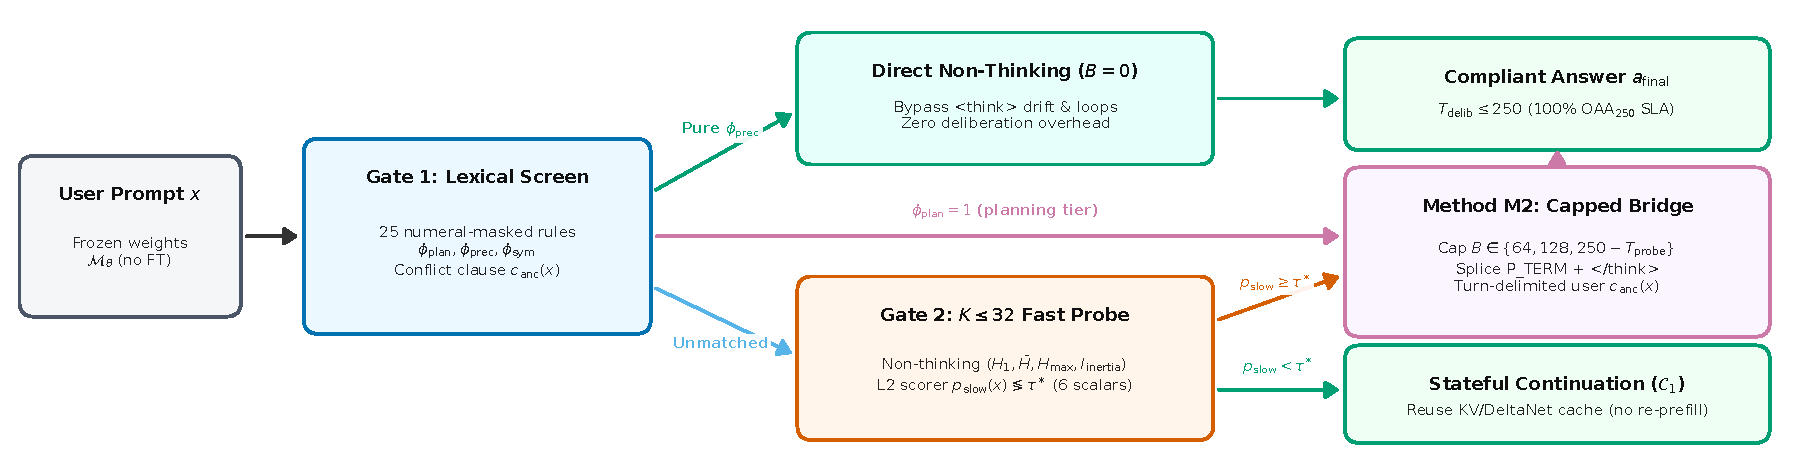
\includegraphics[width=0.98\linewidth]{figures/fig0_cbarr_overview.pdf}
\caption{Overview of training-free \textbf{C-BARR} inference. Gate~1 screens numeral-masked rules in $<1$\,ms, bypassing deliberation on pure precision constraints ($\phi_{\text{prec}}$) and extracting conflict-balanced clauses $c_{\text{anc}}(x)$. Unmatched prompts enter Gate~2's $K \le 32$-token non-thinking probe, either continuing statefully from $\mathcal{C}_1$ or escalating to Method~M2's capped deliberation ($T_{\text{delib}} \le 250$) with turn-delimited post-\texttt{</think>} re-anchoring.}
\label{fig:overview}
\end{figure}

We introduce \textbf{Cascaded Budgeted Adaptive Reasoning Routing (C-BARR)} (Figure~\ref{fig:overview}), a training-free framework operating on frozen weights with six scalar parameters fitted on 120 held-out prompts. Our contributions are:
\begin{enumerate}
    \item \textbf{Stateful cascaded routing and turn-delimited bridging:} We pair a 25-rule numeral-masked lexical screen (\textbf{Gate~1}) and a $K \le 32$-token non-thinking entropy plus Thinking Inertia probe (\textbf{Gate~2}) with tiered caps ($B \in \{64, 128, 250 - T_{\text{probe}}\}$) and \texttt{user}-turn post-\texttt{</think>} re-anchoring (\textbf{Method~M2}), guaranteeing $T_{\text{delib}} \le 250$ while reusing Stage-1 caches.
    \item \textbf{Finite-sample degradation risk control:} We establish split conformal and uniform finite-grid degradation risk bounds for threshold calibration (Proposition~\ref{prop:conformal}), verified across all five models ($\le 1.11\%$ test degradation vs.\ \textbf{B1b} across \texttt{Qwen3.5}).
    \item \textbf{Cross-scale, latency, and OOD gains:} Across \texttt{Qwen3.5-0.8B/2B/4B/9B} and dense \texttt{SmolLM3-3B} \cite{benallal2025smollm3}, C-BARR yields $+47.7$ to $+55.9$\,pp macro-accuracy gains over thinking on hybrid models ($4.59\times$--$5.08\times$ latency speedup), matches dense \texttt{SmolLM3-3B} accuracy at $62.0\%$ token savings ($2.74\times$ speedup), and generalizes zero-shot to 58 unseen \texttt{IFBench} rules ($+29.3$\,pp over \textbf{B1b}, $p = 1.73 \times 10^{-24}$).
    \item \textbf{Architectural mechanics of constraint drift:} Across six counterfactual controls ($n=912$ strict / $n=416$ full \texttt{E\_hurt}) and zero-token state surgeries, we show Gated DeltaNet drift is $96.1\%$ multiplicative recency decay ($95.8\%$ restored via recurrent+conv state blending), whereas dense GQA retains $37.5\%$ global \texttt{<think>} KV interference ($62.5\% \to 86.2\%$ via zero-token \texttt{<think>} KV eviction).
\end{enumerate}

\section{Related work and architectural preliminaries}
\label{sec:related}

\paragraph{Adaptive test-time compute and early stopping.}
Test-time scaling methods control reasoning length via budget forcing \cite{muennighoff2025s1,ma2025nothinking}, trace compression \cite{lorup2026concise9b}, stochastic draft agreement \cite{lee2026dart}, typed multi-budget calibration \cite{ding2026thinkjev}, or intra-trace stopping rules driven by token entropy, attention states, and sequential statistical or PAC/conformal guarantees \cite{yan2026entrocut,xie2026statstop,li2026asag,zeng2025pac,yu2026bpac,wang2026conformal}. However, recent audits show that intra-trace truncation still pays thinking prefill overhead on trivial queries and assumes approximately monotonic accuracy in budget $B$ \cite{aggarwal2025optimalthinkingbench,nguyen2026early}---an assumption violated when thinking actively corrupts formatting constraints. Input-level mode routers instead train external classifiers \cite{li2025pitfalls,yu2026hdm}, probe frozen prefill representations \cite{li2026sonata,varshney2026llmrouter,milios2026scout}, or inspect short non-thinking glimpses \cite{tan2025zerostep,xia2026edrm,ning2026hrbench,zeng2026glimprouter}. C-BARR unifies zero-generation lexical screening with stateful non-thinking probing ($K \in \{1, 4, 8, 16, 32\}$) and bridges the orthogonal gap left by pure routers: preserving instruction fidelity \emph{after} escalated deliberation terminates.

\paragraph{Instruction drift and hybrid linear-attention state dynamics.}
Reasoning-induced instruction forgetting affects negative omissions and structural formatting most acutely \cite{li2025pitfalls,kwon2025reasonif,kumar2026constraint,gamage2026omission,kariyappa2026hierarchy,dong2025ifevalpp}. Existing mitigations steer softmax attention weights \cite{venkateswaran2026spotlight}, repeat prompts \cite{leviathan2025promptrep}, or inject cues ahead of or inside \texttt{<think>} \cite{wu2025intervention,li2026thinkpilot,zhao2026bridging}. Pre-softmax steering is incompatible with hybrid linear-attention models such as \texttt{Qwen3.5}, where $75\%$ of layers replace KV caches with Gated DeltaNet recurrent states \cite{yang2024gateddeltanet,zeng2026linearquery} updated at token $t$ via
\begin{equation}
\label{eq:deltanet}
S_t = \alpha_t S_{t-1}\!\left(I - \beta_t k_t k_t^\top\right) + \beta_t v_t k_t^\top, \qquad \alpha_t \in (0, 1), \; \beta_t \in (0, 1).
\end{equation}
Across $T_{\text{think}} \gg 10^2$ reasoning steps, cumulative gating $\prod_{j=t_{\text{prompt}}+1}^{T} \alpha_j$ exponentially attenuates prompt-encoded formatting features in $S_t$ \cite{zhou2026amnesia}. In contrast, dense GQA models (\texttt{SmolLM3-3B}, 36 full-attention layers with 3:1 NoPE) retain exact prompt keys $[K_{\text{prompt}}, V_{\text{prompt}}]$ indefinitely, but expose response decoding to competitive softmax attention over hundreds of intermediate \texttt{<think>} KV pairs $[K_{\text{think}}, V_{\text{think}}]$. Section~\ref{sec:mechanistic} directly tests both mechanisms.

\section{Cascaded budgeted adaptive reasoning routing (C-BARR)}
\label{sec:method}

Let $\mathcal{M}_\theta$ be a frozen dual-mode language model evaluated on prompt $x$ with binary task verifier $z(x, a_{\text{final}}) \in \{0, 1\}$ and total generated tokens $T_{\text{total}} = T_{\text{probe}} + T_{\text{think}} + T_{\text{inj}} + T_{\text{ans}}$. Under an interactive deliberation service-level agreement (SLA) of $B_{\text{SLA}} = 250$ deliberative tokens ($T_{\text{delib}} = T_{\text{probe}} + T_{\text{think}} \le 250$), we seek a routing and generation policy $\pi$ maximizing efficiency-adjusted linear utility $U_\lambda(x) = z(x) - \lambda (T_{\text{total}}(x) / 250)$ at $\lambda = 0.05$ \cite{aggarwal2025optimalthinkingbench,nguyen2026early}.

\subsection{Gate 1: Numeral-masked lexical screening and conflict-balanced clauses}
Gate~1 applies deterministic regular-expression transducers across the 25 verifiable constraint categories of \citet{zhou2023ifeval}, partitioning matches into compositional \emph{planning} indicators $\phi_{\text{plan}}(x) \in \{0, 1\}$ (10 rules requiring structural counting or multi-section layout, e.g., exact paragraph/sentence counts) and surface \emph{precision} indicators $\phi_{\text{prec}}(x) \in \{0, 1\}$ (5 negative-inhibition rules such as forbidden words/punctuation and 10 local wrapper rules such as JSON, casing, or exact postscripts), disambiguating capital-word count constraints from structural planning. To prevent numeric formatting parameters (e.g., ``at least 300 words'') from triggering false arithmetic escalation, Gate~1 masks unit-bound numerals inside non-question constraint clauses before evaluating multi-number mathematical symbolism $\phi_{\text{sym}}(x) \in \{0, 1\}$.

Gate~1 routes pure precision prompts ($\phi_{\text{prec}} = 1 \land \phi_{\text{plan}} = 0 \land \phi_{\text{sym}} = 0$) directly to non-thinking decoding ($B = 0$), avoiding reasoning-induced inhibition drift at zero probe cost. Prompts with $\phi_{\text{plan}} = 1$ escalate directly to budgeted deliberation ($B = 128$, or $B = 250$ when $\phi_{\text{sym}} = 1$ or multi-clause conflicts occur) and synthesize a compact ($\le 30$-word) anchor clause $c_{\text{anc}}(x)$. When both $\phi_{\text{plan}} = 1$ and $\phi_{\text{prec}} = 1$ (\texttt{ifeval\_conflict}), $c_{\text{anc}}(x)$ allocates balanced spans (\texttt{Structure: <plan> | Format: <prec>}) so verbose negative lists never clip structural targets \cite{zhao2026bridging}.

\subsection{Gate 2: Stateful non-thinking entropy and Thinking Inertia probing}
Prompts with $\phi_{\text{plan}} = \phi_{\text{prec}} = 0$ enter Gate~2, decoding up to $K = 32$ non-thinking tokens while retaining KV/DeltaNet cache $\mathcal{C}_1$. At step $t \in \{1, \dots, T_{\text{probe}}\}$, we record Shannon entropy $H_t = -\sum_{v \in \mathcal{V}} p_t(v) \log p_t(v)$ and an online \emph{Thinking Inertia} indicator $I_{\text{inertia}}(x) \in \{0, 1\}$ capturing spontaneous derivation cues (e.g., ``Step 1:'', ``Let's calculate'') emitted under non-thinking mode \cite{lei2026thinkinginertia,zhu2026savethinking}. Forming $\psi(x) = [H_1, \bar{H}_{1:T_{\text{probe}}}, H_{\max}, I_{\text{inertia}}(x), \phi_{\text{sym}}(x)]^\top \in \mathbb{R}^5$, we fit standardized L2-regularized balanced logistic weights $(w, b)$ ($C = 0.25$) on $\texttt{seed\_60}$ against strict slow-gain targets $y(x) = \mathbb{I}[z_{\text{B1b}}(x) > z_{\text{B0}}(x)]$:
\begin{equation}
\label{eq:gate2}
p_{\text{slow}}(x) = \sigma\!\left(w^\top \psi(x) + b\right), \qquad \text{escalate iff } p_{\text{slow}}(x) \ge \tau^*.
\end{equation}
Threshold $\tau^* \in \mathcal{G}_{29} = \{0.20, 0.225, \dots, 0.90\}$ maximizes empirical utility $\hat{U}_\lambda(\tau)$ on disjoint $\texttt{dev\_60}$ under conservative near-tie selection ($\epsilon = 0.002$). When $p_{\text{slow}}(x) < \tau^*$ without EOS, decoding continues directly from $\mathcal{C}_1$ with zero re-prefill.

\subsection{Method M2: Budgeted termination and turn-delimited post-think bridging}
Escalated queries receive tiered cap $B(x) = 64$ if $p_{\text{slow}}(x) < \tau^* + 0.15 \land \phi_{\text{sym}} = 0$, $B(x) = 128$ for moderate uncertainty or single-clause planning, and $B(x) = 250 - T_{\text{probe}}$ when $H_{\max} \ge \tau_H$ or math/conflict cues appear, strictly bounding $T_{\text{delib}} = T_{\text{probe}} + T_{\text{think}} \le 250$. Unclosed traces at $B(x)$ splice closing phrase \texttt{P\_TERM} before \texttt{</think>} \cite{ma2025nothinking} while preserving Stage-1 state. Whenever $c_{\text{anc}}(x) \neq \emptyset$, Method~M2 closes the assistant turn after \texttt{</think>}, injects a turn-delimited \texttt{user} reminder (\texttt{[Reminder: strictly follow: $c_{\text{anc}}(x)$]}), and opens a fresh empty-think \texttt{assistant} turn capped at $1024$ tokens (\texttt{post\_stripped}), preventing verbatim assistant echoing while placing constraints at zero distance from answer token $a_1$. Auxiliary \textbf{M2-Prec} (outside our confirmatory family) also routes pure $\phi_{\text{prec}}$ items through $B=128$ turn-bridged deliberation.

\begin{proposition}[Finite-sample degradation risk control]
\label{prop:conformal}
Let $\ell_{\mathrm{deg}}(x; \tau) = \max(0, z_{\mathrm{base}}(x) - z_{\mathrm{M2}}(x; \tau)) \in \{0, 1\}$ denote binary accuracy loss of C-BARR relative to baseline $\mathrm{base} \in \{\mathrm{B0}, \mathrm{B1b}\}$, with empirical risk $\hat{R}_n(\tau) = \frac{1}{n}\sum_{i=1}^n \ell_{\mathrm{deg}}(X_i; \tau)$ on $n$ validation examples exchangeable with test draw $X_{n+1}$. (i) For any pre-fixed threshold $\tau$, split conformal prediction guarantees $\mathbb{E}[\ell_{\mathrm{deg}}(X_{n+1}; \tau)] \le \frac{n\hat{R}_n(\tau) + 1}{n + 1}$ \cite{wang2026conformal}. (ii) For data-dependent $\tau^*$ chosen over finite grid $\mathcal{G}_M$ ($|\mathcal{G}_M| = M$), union-bounded Hoeffding concentration guarantees with probability at least $1 - \delta$ over i.i.d.\ validation draws that conditional test risk satisfies
\begin{equation}
\label{eq:conformal}
R(\tau^*) = \mathbb{E}\!\left[\ell_{\mathrm{deg}}(X_{n+1}; \tau^*) \mid \mathcal{D}_{\mathrm{dev}}\right] \le \hat{R}_n(\tau^*) + \sqrt{\frac{\ln(M / \delta)}{2n}}.
\end{equation}
\end{proposition}
The proof (Appendix~\ref{app:proof}) follows directly from rank exchangeability of binary nonconformity indicators for (i) and Hoeffding's inequality union-bounded across $M=29$ candidate thresholds at $\delta=0.05$ for (ii).

\section{Experimental setup}
\label{sec:setup}

\paragraph{Datasets, splits, and deterministic verifiers.}
All splits are frozen at $\text{seed}=42$ with SHA-256 verification and zero UID overlap: $\texttt{seed\_60}$ ($n=60$) and $\texttt{dev\_60}$ ($n=60$) for calibration; $\texttt{eval\_450}$ ($N=450$) across six slices---GSM8K Easy ($n=75$) and Hard ($n=75$) \cite{cobbe2021gsm8k}, CommonsenseQA ($n=150$) \cite{talmor2019commonsenseqa}, and IFEval Planning ($n=60$), Precision ($n=60$), and Conflict ($n=30$) \cite{zhou2023ifeval}; plus counterfactual pools $\texttt{ifeval\_diag\_341\_strict}$ ($n=341$) and $\texttt{ifeval\_diag\_491}$ ($n=491$). Zero-shot OOD transfer is evaluated on $\texttt{allenai/IFBench\_test}$ ($N=300$, 58 unseen rules) \cite{pyatkin2025ifbench}. We pin \texttt{DetectorFactory.seed = 0}, strip \texttt{<think>} channels before grading, audit CoT spillover, and verify Clean-446 sensitivity.

\paragraph{Model backbones, baselines, and statistical protocol.}
We evaluate five open-weight models in \texttt{bfloat16} on $8\times$ NVIDIA L40 (46\,GB) GPUs with Triton \texttt{flash-linear-attention} and CUDA \texttt{causal-conv1d}: four hybrid 3:1 Gated DeltaNet scales (\texttt{Qwen/Qwen3.5-0.8B}, \texttt{2B}, \texttt{4B} primary, \texttt{9B}) \cite{yang2024gateddeltanet,yang2025qwen3} and dense 36-layer GQA \texttt{HuggingFaceTB/SmolLM3-3B} \cite{benallal2025smollm3}, under greedy decoding ($T=0$) plus 3-seed sampling ($T=0.6$) in Appendix~\ref{app:robustness}. Baselines span \textbf{B0} (non-thinking), \textbf{B1a} (prompted CoT), \textbf{B1b} (thinking, $B=2048$), \textbf{B2a} (self-selective prompting), \textbf{B2b} (random escalation), unbudgeted routers \textbf{M1a}--\textbf{M1c}, C-BARR ablations (\textbf{M2-64/128/250}, \textbf{M2-Pre}), full \textbf{M2}, auxiliary \textbf{M2-Prec} and \textbf{M2-512}, and hindsight \textbf{Oracle\_UB}. Testing separates a pre-registered 4-pair confirmatory Holm-Bonferroni family (\textbf{M2} vs.\ \textbf{B1b}, \textbf{B0}, \textbf{B2a}, \textbf{M1c}) from 12-way exploratory Holm ($p_{\text{Holm},12}$), paired with 10,000-resample bootstrap 95\% CIs.

% Auto-generated by scripts/analyze_and_plot.py from frozen matrix outputs
% Table 1: Main C-BARR Comparison (Qwen/Qwen3.5-4B)
\begin{table}[t]
\centering
\caption{Main results across the frozen $N=450$ suite (\texttt{Qwen/Qwen3.5-4B}). Headline evaluation leads with MacroAcc, $U_{0.05}$, $\text{AUC}_{\text{OAA}}$, and Token Savings; $\text{OAA}_{250}$ equals MicroAcc on \textbf{M2} by D13 cap design ($\le 250$ SLA). $^\dagger p_{\text{Holm},12} < 0.05$ vs.\ \textbf{B1b} (exploratory 12-way exact McNemar); $^\ddagger p_{\text{Holm},4} < 0.05$ (pre-registered 4-pair confirmatory family).}
\label{tab:main_results}
\resizebox{\textwidth}{!}{%
\begin{tabular}{lccccccccccc}
\toprule
\textbf{System Variant} & \textbf{GSM-E} & \textbf{GSM-H} & \textbf{CSQA} & \textbf{IFE-Plan} & \textbf{IFE-Prec} & \textbf{IFE-Conf} & \textbf{MacroAcc} $\uparrow$ & $\textbf{OAA}_{250}$ (SLA) $\uparrow$ & $\textbf{AUC}_{\text{OAA}}$ $\uparrow$ & ${U}_{0.05}$ $\uparrow$ & ${\overline{T}}_{\text{tot}}$ / \textbf{Calls} $\downarrow$ \\
\midrule
B0: Always Non-Thinking ($B=0$) & 92.0 & 90.7 & 82.0 & 80.0 & 83.3 & 76.7 & 84.1$^\dagger$ & 84.7 & 84.7 & 78.4 & 312 / 1.00 \\
B1a: Prompted CoT (\textit{Step-by-step}) & 93.3 & 92.0 & 84.0 & 66.7 & 76.7 & 70.0 & 80.4$^\dagger$ & 36.7 & 71.7 & 74.8 & 395 / 1.00 \\
B1b: Always Thinking ($B=2048$) & 56.0 & 44.0 & 41.3 & 11.7 & 21.7 & 6.7 & 30.2 & 0.2 & 18.1 & 0.6 & 1735 / 1.00 \\
B2a: Self-Selective Prompting & 97.3 & 94.7 & 80.7 & 80.0 & 75.0 & 66.7 & 82.4$^\dagger$ & 51.6 & 75.3 & 77.8 & 310 / 1.00 \\
B2b: Budget-Matched Random Esc. & 85.3 & 84.0 & 70.7 & 71.7 & 70.0 & 53.3 & 72.5$^\dagger$ & 66.2 & 70.4 & 61.4 & 639 / 1.23 \\
\midrule
M1a: Regex Constraint Router (Gate 1) & 66.7 & 49.3 & 82.0 & 16.7 & 76.7 & 20.0 & 51.9$^\dagger$ & 43.8 & 52.2 & 40.9 & 979 / 1.00 \\
M1b: Fast Entropy + Inertia Router (Gate 2) & 92.0 & 90.7 & 79.3 & 66.7 & 78.3 & 60.0 & 77.8$^\dagger$ & 77.1 & 78.7 & 71.6 & 429 / 1.08 \\
M1c: Dual-Signal Cascade (Gate 1 + Gate 2) & 92.0 & 88.0 & 79.3 & 15.0 & 78.3 & 20.0 & 62.1$^\dagger$ & 65.6 & 67.8 & 56.6 & 680 / 1.04 \\
\midrule
M2-64: C-BARR Fixed Cap ($B=64$ + Post-Anc.) & 92.0 & 90.7 & 81.3 & 80.0 & 81.7 & 80.0 & 84.3$^\dagger$ & 84.4 & 83.8 & 77.8 & 335 / 1.04 \\
M2-128: C-BARR Fixed Cap ($B=128$ + Post-Anc.) & 92.0 & 90.7 & 81.3 & 83.3 & 83.3 & 76.7 & 84.6$^\dagger$ & 84.9 & 83.6 & 77.8 & 355 / 1.04 \\
M2-250: C-BARR Fixed Cap ($B=250$ + Post-Anc.) & 92.0 & 90.7 & 81.3 & 85.0 & 81.7 & 76.7 & 84.6$^\dagger$ & 84.9 & 82.5 & 77.3 & 380 / 1.04 \\
M2-Pre: Tiered $\{64,128,250\}$ + Pre-Anc. & 92.0 & 89.3 & 81.3 & 83.3 & 81.7 & 70.0 & 82.9$^\dagger$ & 84.0 & 82.6 & 76.7 & 364 / 1.04 \\
\textbf{M2: Full C-BARR ($\{64,128,250\}$ + Post-Anc.)} & 92.0 & 90.7 & 81.3 & 83.3 & 83.3 & 76.7 & 84.6$^{\dagger\ddagger}$ & 84.9 & 83.4 & 77.7 & 360 / 1.04 \\
M2-Prec: C-BARR Aux.\ ($\phi_{\text{prec}} \to \text{M2-128}$) & 92.0 & 90.7 & 81.3 & 83.3 & 91.7 & 73.3 & 85.4 & 85.8 & 83.6 & 78.1 & 384 / 1.04 \\
M2-512: C-BARR Aux.\ Cap ($B=512$, R3) & 92.0 & 90.7 & 82.0 & 86.7 & 81.7 & 83.3 & 86.1 & 65.6 & 80.7 & 76.9 & 445 / 1.04 \\
\midrule
\textit{Instance-Level Oracle\_UB} & 97.3 & 98.7 & 92.7 & 93.3 & 93.3 & 90.0 & 94.2 & 92.2 & 92.3 & 88.4 & 300 / 1.00 \\
\bottomrule
\end{tabular}}
\end{table}


\section{Main accuracy, SLA compliance, and latency results}
\label{sec:main_results}

Table~\ref{tab:main_results} and Figure~\ref{fig:pareto} report primary results on \texttt{Qwen/Qwen3.5-4B} ($N=450$). Always-thinking (\textbf{B1b}) incurs $58.4\%$ 4-gram loops and $63.8\%$ budget exhaustion, depressing macro-accuracy to $30.2\%$ at $1735$ tokens. Full \textbf{C-BARR (M2)} reaches $84.6\%$ macro-accuracy---gaining $+54.3$\,pp over \textbf{B1b} (95\% CI $[+49.2, +59.3]$\,pp, $226\!:\!3$ wins, $p_{\text{Holm},4} = 1.86 \times 10^{-62}$) while cutting tokens by $79.2\%$ ($360$ vs.\ $1735$) and lifting $U_{0.05}$ by $+77.0$\,pp ($[+71.6, +82.4]$\,pp). Clean-446 filtering shifts macro-accuracy by $\le 0.36$\,pp on \texttt{4B} ($\le 0.48$\,pp across all backbones).

\begin{figure}[t]
\centering
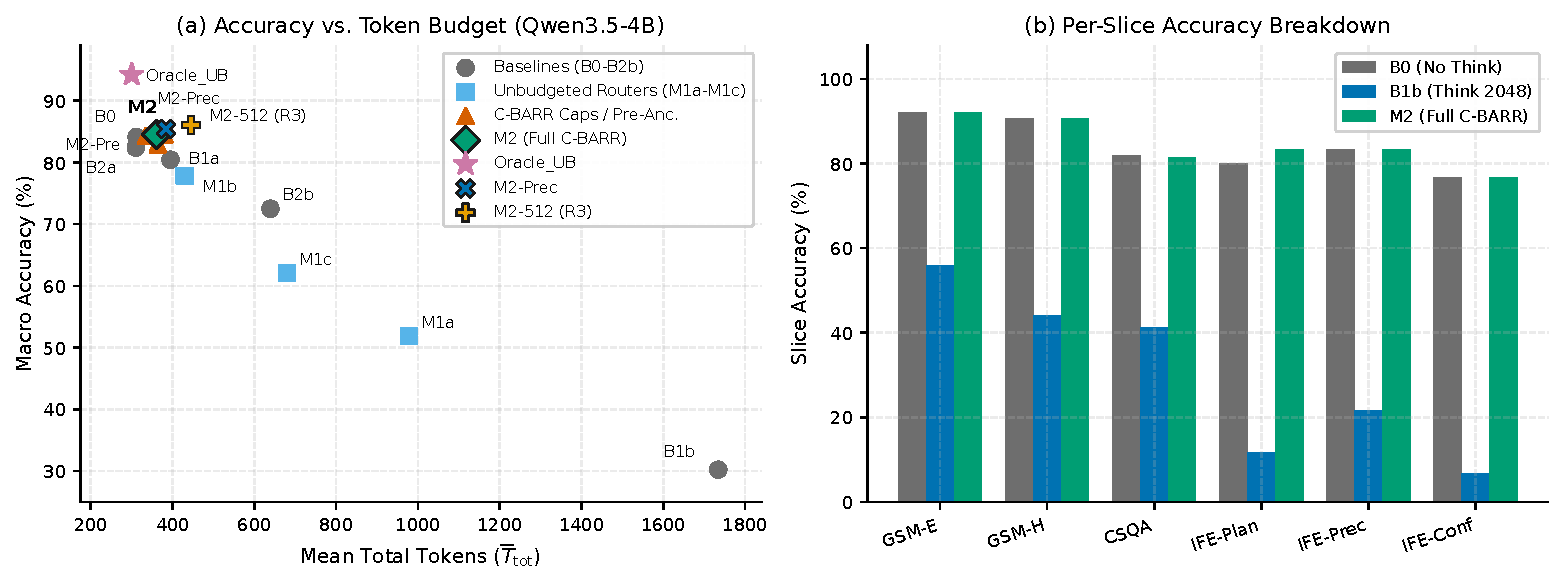
\includegraphics[width=0.96\linewidth]{figures/fig1_pareto_frontier.pdf}
\caption{Primary \texttt{Qwen3.5-4B} evaluation ($N=450$): (a) accuracy--token Pareto frontier across baselines, routers, C-BARR variants, and \texttt{Oracle\_UB}; (b) per-slice accuracy showing C-BARR eliminates \textbf{B1b}'s collapse on planning, precision, and conflict constraints.}
\label{fig:pareto}
\end{figure}

\begin{figure}[t]
\centering
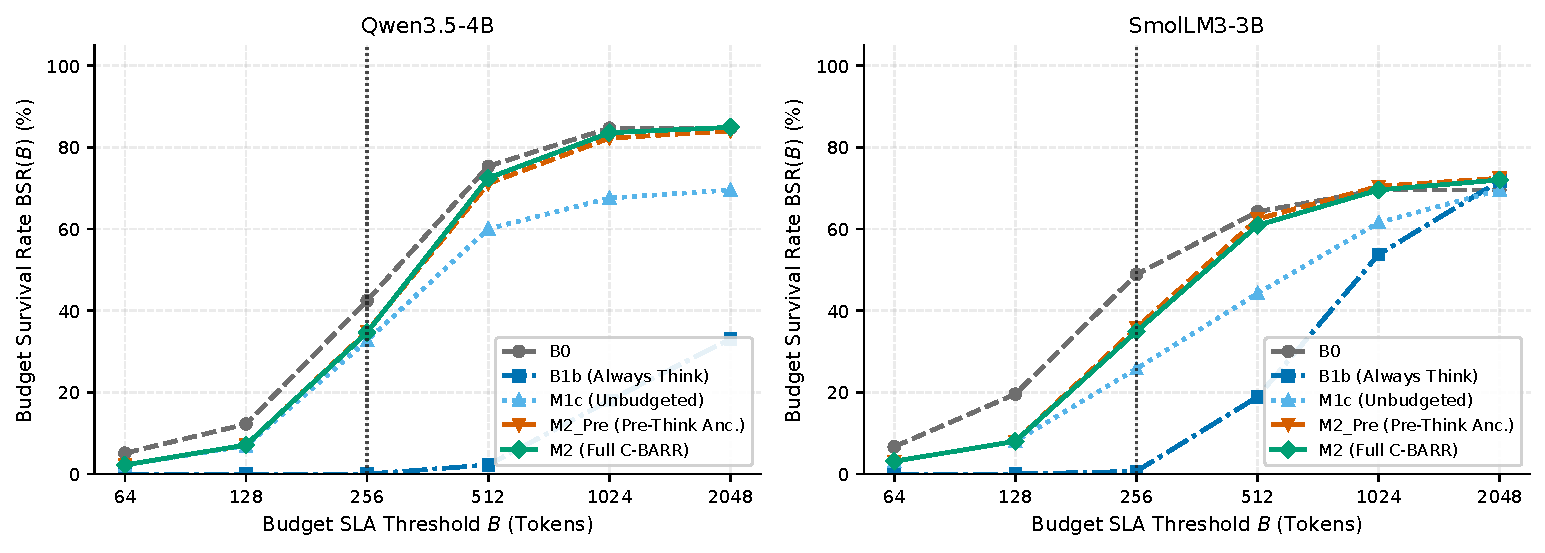
\includegraphics[width=0.94\linewidth]{figures/fig2_bsr_sla_curve.pdf}
\caption{Budget Survival Rate $\text{BSR}(B)$ across total-token thresholds $B \in \{64, \dots, 2048\}$ on \texttt{Qwen3.5-4B} and dense \texttt{SmolLM3-3B} (vertical dotted line marks $B \le 250$ cap).}
\label{fig:bsr_sla}
\end{figure}

\paragraph{Why routing without budgeted post-anchoring fails.}
Comparing unbudgeted cascade \textbf{M1c} ($62.1\%$, $680$ tokens) with \textbf{M2} ($84.6\%$, $360$ tokens) yields $+22.4$\,pp ($66\!:\!0$ wins, $p_{\text{Holm},4} = 8.13 \times 10^{-20}$) and $47.0\%$ token savings: \textbf{M1c} preserves GSM8K ($92.0\% / 88.0\%$) and pure precision ($78.3\%$), but escalated planning items (\texttt{IFE-Plan} $15.0\%$, \texttt{IFE-Conf} $20.0\%$) still suffer unbridged thinking drift. Post-\texttt{</think>} turn bridging (\textbf{M2}) also beats pre-\texttt{</think>} injection (\textbf{M2-Pre}, $82.9\%$) by $+6.7$\,pp on \texttt{IFE-Conf} ($76.7\%$ vs.\ $70.0\%$). Auxiliary \textbf{M2-Prec} lifts \texttt{IFE-Prec} to $91.7\%$ ($85.4\%$ macro-accuracy), and $B=512$ (\textbf{M2-512}) reaches $86.1\%$. Overall, \textbf{M2} retains $89.7\%$ of hindsight \textbf{Oracle\_UB} ($94.2\%$) at $1.20\times$ oracle tokens ($360$ vs.\ $300$) while satisfying Proposition~\ref{prop:conformal} ($0.67\%$ test degradation vs.\ \textbf{B1b} $\le 3.3\%$ CRC bound; $1.11\%$ vs.\ \textbf{B0}).

\paragraph{Operational SLA survival and wall-clock latency.}
Under deliberation SLA $T_{\text{delib}} \le 250$ (Figure~\ref{fig:bsr_sla}), \textbf{M2} achieves $\text{OAA}_{250} = 84.9\%$ vs.\ $0.2\%$ for \textbf{B1b} and $51.6\%$ for \textbf{B2a}. On NVIDIA L40 GPUs (Table~\ref{tab:latency_compute}), \textbf{M2} cuts mean per-query latency on \texttt{Qwen3.5-4B} from $63.62$\,s (P95 $77.06$\,s) to $12.75$\,s (P95 $35.97$\,s), delivering a \textbf{$4.99\times$ wall-clock speedup} ($4.59\times$--$5.08\times$ across \texttt{Qwen3.5}).

% Auto-generated by scripts/analyze_and_plot.py from frozen matrix outputs
% Table 2: Cross-Scale 4-Regime Flip Audit, Loop Pathology, and C-BARR Recovery
\begin{table}[t]
\centering
\caption{Cross-scale 4-regime disagreement audit (\textbf{B0} vs.\ \textbf{B1b} on $N=450$), loop rate, budget exhaustion rate ($B=2048$), and \textbf{M2} token savings.}
\label{tab:scale_and_pathology}
\resizebox{\textwidth}{!}{%
\begin{tabular}{llcccccccc}
\toprule
\textbf{Model Backbone} & \textbf{Mixer Architecture} & \textbf{\% Helped} & \textbf{\% Hurt} & \textbf{B1b Loop\%} $\downarrow$ & \textbf{B1b Exh.\%} $\downarrow$ & \textbf{M2 Loop\%} $\downarrow$ & \textbf{B1b Macro} & \textbf{M2 Macro} $\uparrow$ & \textbf{Token Sav.\%} $\uparrow$ \\
\midrule
\texttt{Qwen3.5-0.8B} & 18 DeltaNet + 6 Attn & 0.4 & 52.7 & 96.4 & 96.0 & 16.7 & 2.7 & 53.6 & 78.2 \\
\texttt{Qwen3.5-2B} & 18 DeltaNet + 6 Attn & 1.1 & 52.7 & 82.4 & 80.2 & 7.6 & 13.7 & 69.6 & 79.7 \\
\texttt{Qwen3.5-4B} & 24 DeltaNet + 8 Attn & 0.7 & 50.0 & 58.4 & 63.8 & 2.7 & 30.2 & 84.6 & 79.2 \\
\texttt{Qwen3.5-9B} & 24 DeltaNet + 8 Attn & 0.9 & 43.8 & 51.3 & 53.1 & 2.4 & 38.3 & 86.0 & 77.2 \\
\midrule
\texttt{SmolLM3-3B} & 36 Full GQA (3:1 NoPE) & 13.6 & 9.6 & 32.0 & 11.3 & 9.6 & 69.4 & 68.5 & 62.0 \\
\bottomrule
\end{tabular}}
\end{table}


\section{Cross-scale pathology and dense-attention parity}
\label{sec:scale}

Table~\ref{tab:scale_and_pathology} audits 4-regime behavioral flips between \textbf{B0} and \textbf{B1b} across five backbones. Across the \texttt{Qwen3.5} hybrid family (\texttt{0.8B} $\to$ \texttt{9B}), scaling model capacity reduces greedy 4-gram repetition loops from $96.4\%$ to $51.3\%$, yet unbudgeted thinking remains overwhelmingly net-harmful across all four scales ($43.8\%$--$52.7\%$ Hurt vs.\ $0.4\%$--$1.1\%$ Helped). C-BARR consistently eliminates budget exhaustion ($0\%$ across all models), cuts repetition loops to $2.4\%$--$16.7\%$, and delivers $+50.9$\,pp (\texttt{0.8B}, $p_{\text{Holm},4}=2.6 \times 10^{-67}$), $+55.9$\,pp (\texttt{2B}, $p_{\text{Holm},4}=2.7 \times 10^{-64}$), $+54.3$\,pp (\texttt{4B}), and $+47.7$\,pp (\texttt{9B}, $p_{\text{Holm},4}=2.5 \times 10^{-50}$) macro-accuracy gains at $77.2\%$--$79.7\%$ token savings ($91.5\%$ Oracle retention on \texttt{9B}). Notably, prompt-only self-selection (\textbf{B2a}) degrades at both smaller and larger scales, trailing \textbf{M2} by $+15.2$\,pp on \texttt{0.8B} ($p_{\text{Holm},4}=4.0 \times 10^{-6}$), $+8.6$\,pp on \texttt{2B} (mid-$p_{\text{Holm},4}=0.040$), and $+7.6$\,pp on \texttt{9B} ($p_{\text{Holm},4}=0.0035$).

On dense 36-layer GQA \texttt{SmolLM3-3B}, \textbf{B1b} terminates reliably ($11.3\%$ exhaustion) and genuinely aids multi-step arithmetic ($13.6\%$ Helped vs.\ $9.6\%$ Hurt, lifting GSM8K-Hard from $72.0\%$ to $89.3\%$), yet still degrades \texttt{IFE-Prec} ($80.0\% \to 71.7\%$) and \texttt{IFE-Conf} ($40.0\% \to 30.0\%$) while failing tight SLAs ($\text{OAA}_{250}=3.6\%$). C-BARR (\textbf{M2} $68.5\%$; \textbf{M2-Prec} $69.9\%$) maintains statistical macro-accuracy parity with \textbf{B1b} ($69.4\%$, $-0.9$\,pp, 95\% CI $[-5.7, +3.7]$\,pp, $p=0.52$) while saving $62.0\%$ tokens ($371$ vs.\ $977$, $2.74\times$ latency speedup), improving $U_{0.05}$ by $+10.6$\,pp ($[+6.1, +15.0]$\,pp), lifting $\text{OAA}_{250}$ by $+68.4$\,pp, and recovering $+10.0$\,pp on both \texttt{IFE-Prec} ($81.7\%$) and \texttt{IFE-Conf} ($40.0\%$).

% Auto-generated by scripts/analyze_and_plot.py from frozen matrix outputs
% Table 3: Section 6 Causal Diagnostic Control on E_hurt
\begin{table}[t]
\centering
\caption{Strict prompt-level recovery (\% and exact $k/n$) on held-out IFEval ``Hurt'' prompts comparing Trace Stripping vs.\ Post-Think Constraint Re-Anchoring. Pooled (\texttt{diag\_491}): A1=100.0\% (416/416), B2a=89.7\% (373/416), $p_{\text{mid},\text{B2a vs B1b}}=5.2e-113$.}
\label{tab:diagnostic_control}
\resizebox{\textwidth}{!}{%
\begin{tabular}{llcccccc}
\toprule
\textbf{Intervention Condition (Fixed $t_{\text{think}}$)} & \textbf{Causal Factor Isolated} & \multicolumn{3}{c}{\textbf{Qwen3.5-4B (DeltaNet, $n=336$)}} & \multicolumn{3}{c}{\textbf{SmolLM3-3B (Dense, $n=80$)}} \\
\cmidrule(lr){3-5} \cmidrule(lr){6-8}
 & & \textbf{All ($k/n$)} & \textbf{Inhib.} & \textbf{Struct.} & \textbf{All ($k/n$)} & \textbf{Inhib.} & \textbf{Struct.} \\
\midrule
B1b: Unmodified \texttt{<think>} ($|t_{\text{think}}|$) & Baseline failure state (0\%) & 0.0 (0/336) & 0.0 & 0.0 & 0.0 (0/80) & 0.0 & 0.0 \\
\textbf{Control A1: Trace Stripping} ($0$ toks) & Deletes \texttt{<think>}; removes decay + interference & 100.0 (336/336) & 100.0 & 100.0 & 100.0 (80/80) & 100.0 & 100.0 \\
\textbf{Control B2a: Post-Think Constraint Re-Anchor (Stripped)} & Keeps \texttt{<think>}; restores post-\texttt{</think>} recency & 96.1 (323/336) & 97.8 & 98.1 & 62.5 (50/80) & 59.0 & 86.0 \\
\midrule
Control B1: Pre-\texttt{</think>} Clause Re-Anchor & Tests pre- vs.\ post-\texttt{</think>} tag locus & 95.5 (321/336) & 98.5 & 96.8 & 58.8 (47/80) & 66.7 & 81.4 \\
Control B2b: Post-\texttt{</think>} Unstripped Visible Prefill & Quantifies wrapper verifier corruption & 49.4 (166/336) & 35.1 & 67.1 & 33.8 (27/80) & 30.8 & 51.2 \\
Control A2: Length-Matched Math Filler ($|t_{\text{think}}|$) & Keeps distance; removes task priming & 70.2 (236/336) & 70.9 & 83.2 & 60.0 (48/80) & 56.4 & 79.1 \\
Control B3: Intra-Trace Cut (No Re-Anchor) & Halves distance; keeps early priming & 86.3 (290/336) & 92.5 & 91.0 & 62.5 (50/80) & 64.1 & 81.4 \\
\midrule
\textit{Derived Recency-Decay Share ($\rho_{\text{recency}}$, \%)} & $R_{\text{post}}/R_{\text{strip}}$ & \multicolumn{3}{c}{96.1} & \multicolumn{3}{c}{62.5} \\
\textit{Residual Semantic Interference ($\rho_{\text{interf}}$, \%)} & $(R_{\text{strip}}-\max(R_{\text{post}},R_{\text{pre}}))/R_{\text{strip}}$ & \multicolumn{3}{c}{3.9} & \multicolumn{3}{c}{37.5} \\
\bottomrule
\end{tabular}}
\end{table}


\section{Causal attribution, state-space restoration, and OOD robustness}
\label{sec:mechanistic}

\subsection{Counterfactual dissection of recency decay versus semantic interference}
To isolate \emph{why} reasoning traces break constraints, Table~\ref{tab:diagnostic_control} and Figure~\ref{fig:ehurt} evaluate six exact-prefix counterfactual interventions on held-out IFEval ``Hurt'' instances ($E_{\text{hurt}} = \{x : z_{\text{B0}}(x)=1 \land z_{\text{B1b}}(x)=0\}$). Deleting the \texttt{<think>} trace (\textbf{Control~A1}) defines the $100\%$ recovery ceiling. Keeping the exact \texttt{<think>} trace intact while appending our turn-delimited post-\texttt{</think>} reminder (\textbf{Control~B2a}) recovers \textbf{$96.1\%$ ($323/336$, 95\% Wilson CI $[93.5\%, 97.7\%]$)} on \texttt{Qwen3.5-4B}---and $90.3\%$ ($771/854$, $p_{\text{mid}} = 8.1 \times 10^{-233}$) pooled across all four \texttt{Qwen3.5} backbones on strictly disjoint $\texttt{diag\_341\_strict}$---attributing $\rho_{\text{recency}} = 96.1\%$ of hybrid constraint failures to context recency decay and only $\rho_{\text{interf}} = 3.9\%$ to irreversible trace interference. Swapping task thoughts for length-matched math derivations (\textbf{A2}, $70.2\%$) or halving trace length without an anchor (\textbf{B3}, $86.3\%$) confirms smooth decay with token distance, whereas injecting an \emph{unstripped} reminder directly into the assistant prefix (\textbf{B2b}) plunges recovery to $49.4\%$ ($35.1\%$ on negative inhibition) due to verbatim reminder echoing (verbatim examples in Appendix~\ref{app:qualitative_impacts}). Conversely, on dense \texttt{SmolLM3-3B} ($n=80$), \textbf{B2a} plateaus at $62.5\%$ ($59.0\%$ inhibition), leaving $\rho_{\text{interf}} = 37.5\%$ unrecovered by text re-anchoring alone.

\begin{figure}[t]
\centering
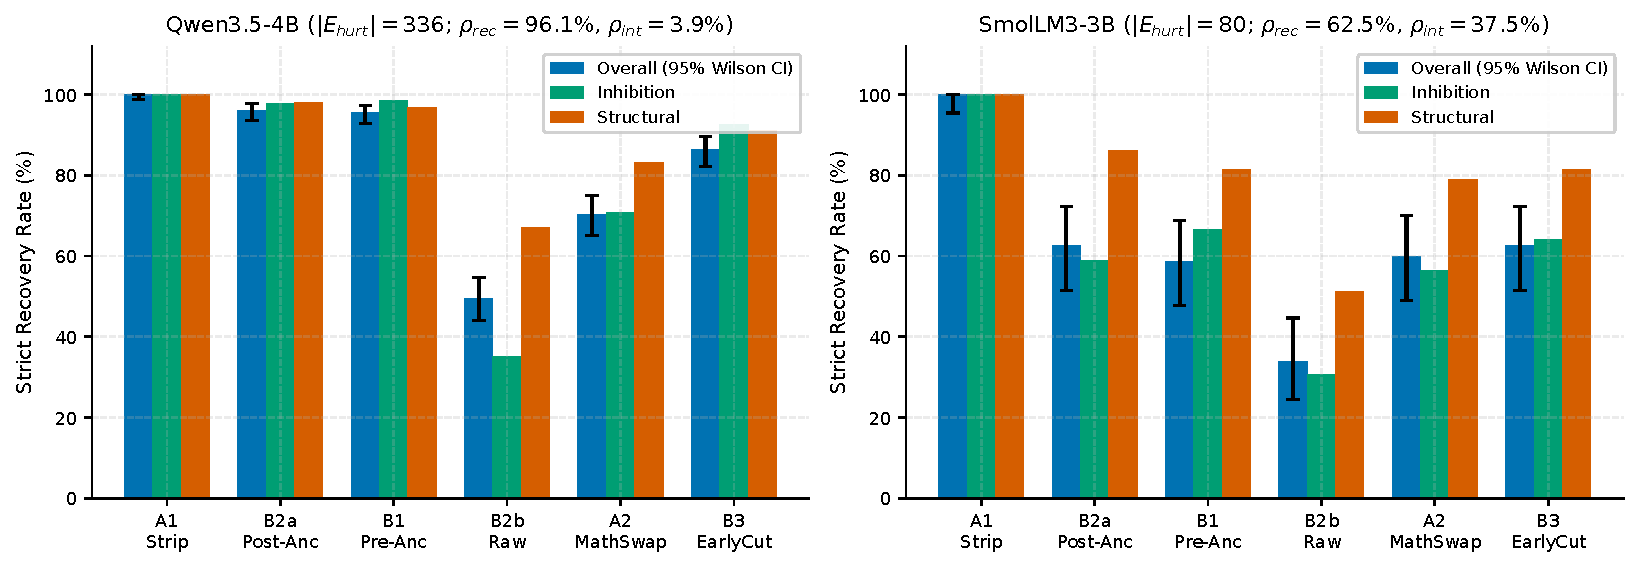
\includegraphics[width=0.96\linewidth]{figures/fig3_ehurt_causal_recovery.pdf}
\caption{Counterfactual $E_{\text{hurt}}$ strict recovery rates (with 95\% Wilson CIs) across Controls~A1--B3, contrasting recency-dominated Gated DeltaNet (\texttt{Qwen3.5-4B}, $\rho_{\text{rec}}=96.1\%$) against interference-heavy dense GQA (\texttt{SmolLM3-3B}, $\rho_{\text{int}}=37.5\%$).}
\label{fig:ehurt}
\end{figure}

\begin{figure}[t]
\centering
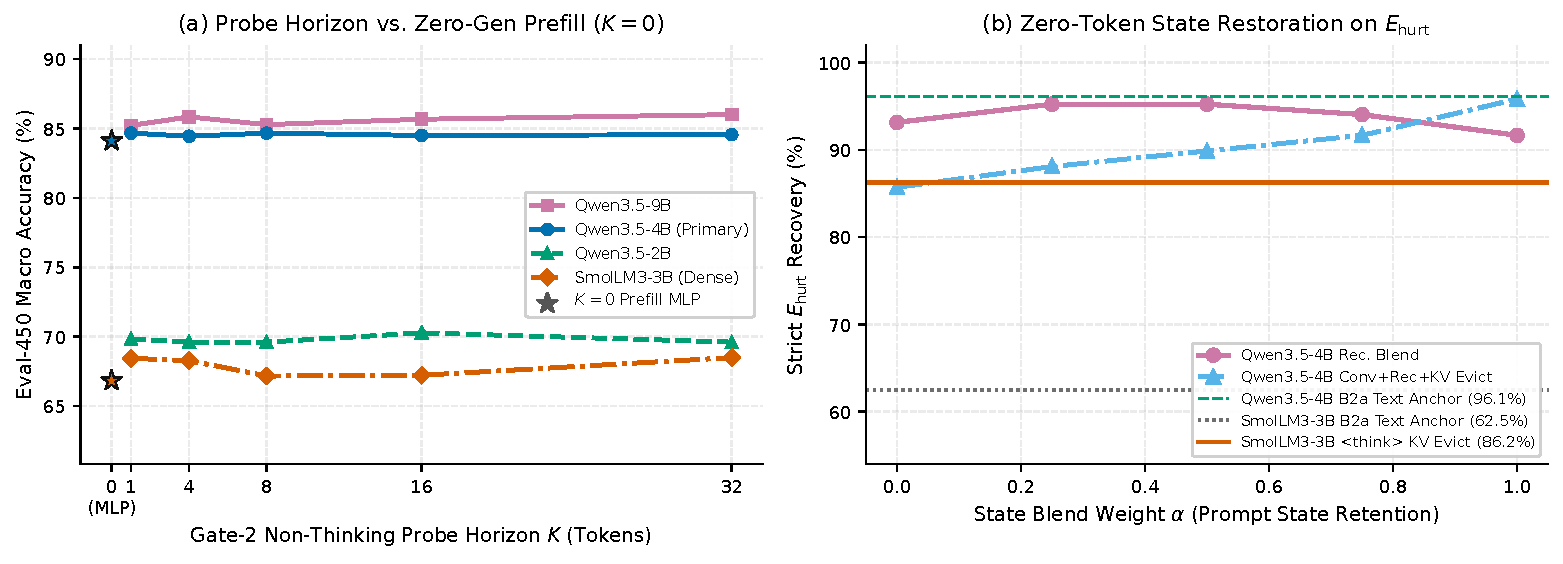
\includegraphics[width=0.98\linewidth]{figures/fig4_horizons_and_w7.pdf}
\caption{Mechanistic ablations: (a) Gate-2 non-thinking probe horizon sweep $K \in \{1, 4, 8, 16, 32\}$ versus zero-generation prefill MLP ($K=0$); (b) zero-token $E_{\text{hurt}}$ recovery via Gated DeltaNet state interpolation ($\alpha \in [0, 1]$) and dense \texttt{<think>} KV cache eviction.}
\label{fig:w7_horizons}
\end{figure}

\subsection{Zero-token state-space restoration across DeltaNet and dense KV caches}
Figure~\ref{fig:w7_horizons}(b) (full sweep in Appendix Table~\ref{tab:extensions_w7}) tests whether constraint compliance can be restored \emph{in state space with zero reminder tokens}. On \texttt{Qwen3.5-4B} ($n=336$), linearly interpolating Gated DeltaNet fast-weight matrices between post-thinking state $S_{\text{think}}$ and clean post-prompt state $S_{\text{prompt}}$ via $S_{\text{blend}} = (1-\alpha)S_{\text{think}} + \alpha S_{\text{prompt}}$ lifts recovery to $95.2\%$ at $\alpha \in \{0.25, 0.50\}$, while jointly restoring 1D short-convolution states and evicting full-attention \texttt{<think>} KV entries reaches \textbf{$95.8\%$ ($98.5\%$ inhibition, $98.7\%$ structural)} at $\alpha = 1.00$---matching text-level \textbf{B2a} ($96.1\%$) with zero injected tokens. Strikingly, on dense \texttt{SmolLM3-3B} ($n=80$), evicting \texttt{<think>} KV cache entries after \texttt{</think>} while keeping prompt KV entries intact jumps recovery from \textbf{$62.5\%$ (\textbf{B2a}) to $86.2\%$ ($94.9\%$ inhibition)} without adding a single token. Together, these interventions prove our architectural hypothesis: linear-attention layers lose constraints by multiplicative fast-weight overwriting (Equation~\ref{eq:deltanet}), whereas dense softmax models retain prompt keys but suffer direct attention competition from intermediate \texttt{<think>} keys.

\subsection{Probe horizons, paraphrase probing, and unseen IFBench generalization}
Figure~\ref{fig:w7_horizons}(a) shows that early non-thinking glimpses carry strong routing signal \cite{zeng2026glimprouter}: $K=1$ token already attains $84.7\%$ macro-accuracy on \texttt{Qwen3.5-4B}, while $K=32$ provides modest gains at larger scale (\texttt{9B}: $85.2\% \to 86.0\%$) and stabilizes threshold calibration across regularizers $C \in \{0.1, 0.25, 0.5, 1.0\}$ ($\le 0.2$\,pp variance on \texttt{4B}/\texttt{9B}/\texttt{SmolLM3}; Appendix Table~\ref{tab:appendix_b_robustness}). Replacing lexical regexes with a lightweight multi-head MLP over frozen mid-layer prefill activations ($K=0$) achieves $84.1\%$ macro-accuracy on \texttt{4B} and outperforms regex screening under \texttt{IFEval++}-style surface paraphrasing \cite{dong2025ifevalpp} ($82.6\%$ vs.\ $78.9\%$ Precision F1; $81.6\%$ vs.\ $69.0\%$ recall). Finally, applying frozen \texttt{Qwen3.5-4B} C-BARR with \emph{zero recalibration} to $\texttt{allenai/IFBench\_test}$ ($N=300$, 58 unseen rules; Appendix~\ref{app:robustness}) improves strict prompt accuracy from $2.0\%$ (\textbf{B1b}, $2034$ tokens) and $28.7\%$ (\textbf{B0}, $386$ tokens) to \textbf{$31.3\%$ (\textbf{M2}, $443$ tokens)} ($+29.3$\,pp over \textbf{B1b}, exact McNemar $p = 1.73 \times 10^{-24}$, $78.2\%$ token savings), gaining $+6.9$\,pp over \textbf{B0} on Gate-1 triggered items ($35.3\%$ vs.\ $28.5\%$, $n=116$) while preventing thinking collapse on the $184$ prompts matching zero lexical templates ($28.8\%$ vs.\ $1.6\%$).

\section{Limitations and conclusion}
\label{sec:limitations}

\paragraph{Limitations.}
First, C-BARR enforces an interactive deliberation SLA ($B \le 250$, or $B \le 512$ in Contingency~R3). On tasks where models genuinely require multi-hundred-token derivations---such as \texttt{SmolLM3-3B} on GSM8K-Hard ($72.0\%$ under \textbf{M2} vs.\ $89.3\%$ under \textbf{B1b} at $977$ tokens) or Olympiad-level mathematics and code synthesis---tight caps trade ceiling accuracy for latency; deploying C-BARR in those domains requires pairing higher escalation tiers ($B \ge 2048$) with our post-\texttt{</think>} turn bridge or KV/state restoration. Second, Gate~1's deterministic regexes lose recall under heavy paraphrase ($69.0\%$ recall on \texttt{IFEval++}), motivating our prefill MLP probe ($81.6\%$ recall) when hidden states are accessible. Third, $3.9\%$--$13.8\%$ residual semantic interference persists even after state restoration when flawed reasoning commitments carry across turn boundaries.

\paragraph{Conclusion.}
We presented C-BARR, a training-free routing and post-deliberation state-bridging framework that eliminates overthinking collapse while preserving strict constraint compliance across hybrid linear-attention and dense reasoning models, achieving $4.6\times$--$5.1\times$ wall-clock speedups on \texttt{Qwen3.5} and exposing the distinct state-space mechanics of constraint forgetting.

\begin{ack}
Funding disclosures and acknowledgments are omitted in the anonymized submission per NeurIPS guidelines and will be provided in the camera-ready version.
\end{ack}

{\small
\bibliographystyle{plainnat}
\bibliography{references}
}

%%%%%%%%%%%%%%%%%%%%%%%%%%%%%%%%%%%%%%%%%%%%%%%%%%%%%%%%%%%%
\clearpage
\appendix

\section{Theoretical proof, algorithm specification, and conformal audit}
\label{app:proof}

\subsection{Complete proof of Proposition~\ref{prop:conformal}}
\begin{proof}
Fix a baseline policy $\mathrm{base} \in \{\mathrm{B0}, \mathrm{B1b}\}$ and define the bounded binary pairwise degradation indicator $\ell_i(\tau) = \ell_{\mathrm{deg}}(X_i; \tau) = \max(0, z_{\mathrm{base}}(X_i) - z_{\mathrm{M2}}(X_i; \tau)) \in \{0, 1\}$ for calibration examples $i \in \{1, \dots, n\}$ ($\mathcal{D}_{\mathrm{dev}} = \texttt{dev\_60}$, $n=60$) and future test draw $X_{n+1}$. Note that Gate~2's logistic direction $w$ and intercept $b$ are fitted solely on disjoint $\texttt{seed\_60}$, so the mapping $x \mapsto \ell_{\mathrm{deg}}(x; \tau)$ is fixed prior to observing $\mathcal{D}_{\mathrm{dev}} \cup \{X_{n+1}\}$.

\emph{Part (i): Split conformal expectation risk bound.} Under exchangeability of $(X_1, \dots, X_n, X_{n+1})$ for any pre-specified threshold $\tau$, the random variables $(\ell_1(\tau), \dots, \ell_n(\tau), \ell_{n+1}(\tau)) \in \{0, 1\}^{n+1}$ are exchangeable. Let $S_{n+1}(\tau) = \sum_{i=1}^{n+1} \ell_i(\tau)$ denote their total sum. By symmetry across the $n+1$ exchangeable coordinates, conditional on $S_{n+1}(\tau)$, each coordinate has identical conditional expectation $\mathbb{E}[\ell_{n+1}(\tau) \mid S_{n+1}(\tau)] = \frac{S_{n+1}(\tau)}{n+1}$. Since $\ell_{n+1}(\tau) \le 1$ almost surely, $S_{n+1}(\tau) = n\hat{R}_n(\tau) + \ell_{n+1}(\tau) \le n\hat{R}_n(\tau) + 1$. Taking marginal expectations yields the exact finite-sample conformal risk bound \cite{wang2026conformal}:
\begin{equation}
\mathbb{E}\!\left[\ell_{\mathrm{deg}}(X_{n+1}; \tau)\right] = \mathbb{E}\!\left[\frac{n\hat{R}_n(\tau) + \ell_{n+1}(\tau)}{n+1}\right] \le \frac{n\,\mathbb{E}[\hat{R}_n(\tau)] + 1}{n + 1},
\end{equation}
with plug-in conformal estimator $\hat{B}_{\mathrm{CRC}}(\tau) = \frac{n\hat{R}_n(\tau) + 1}{n + 1}$.

\emph{Part (ii): Uniform concentration over data-dependent $\tau^* \in \mathcal{G}_M$.} Suppose $\mathcal{D}_{\mathrm{dev}} = (X_1, \dots, X_n)$ is drawn i.i.d.\ from test distribution $\mathcal{P}$, and let $R(\tau) = \mathbb{E}_{X \sim \mathcal{P}}[\ell_{\mathrm{deg}}(X; \tau)] \in [0, 1]$. For any fixed $\tau \in \mathcal{G}_M$, $\ell_1(\tau), \dots, \ell_n(\tau)$ are independent bounded random variables in $[0, 1]$ with mean $R(\tau)$. By Hoeffding's one-sided inequality, for any $\epsilon > 0$,
\begin{equation}
\Pr_{\mathcal{D}_{\mathrm{dev}}}\!\left(R(\tau) - \hat{R}_n(\tau) > \epsilon\right) \le \exp\!\left(-2n\epsilon^2\right).
\end{equation}
Applying the union bound over the finite threshold grid $\mathcal{G}_M$ ($|\mathcal{G}_M| = M = 29$ thresholds in $[0.20, 0.90]$) gives
\begin{equation}
\Pr_{\mathcal{D}_{\mathrm{dev}}}\!\left(\exists\,\tau \in \mathcal{G}_M : R(\tau) - \hat{R}_n(\tau) > \epsilon\right) \le \sum_{\tau \in \mathcal{G}_M} \exp\!\left(-2n\epsilon^2\right) = M \exp\!\left(-2n\epsilon^2\right).
\end{equation}
Setting $M \exp(-2n\epsilon^2) = \delta$ solves to $\epsilon = \sqrt{\frac{\ln(M/\delta)}{2n}}$. Since $\tau^* \in \mathcal{G}_M$ on every realization of $\mathcal{D}_{\mathrm{dev}}$, with probability at least $1 - \delta$ ($0.95$ at $\delta = 0.05$), $R(\tau^*) \le \hat{R}_n(\tau^*) + \sqrt{\frac{\ln(M/\delta)}{2n}}$.
\end{proof}

\begin{table}[h]
\centering
\caption{Algorithm~\ref{alg:cbarr}: Training-free C-BARR online inference and stateful turn-bridged termination.}
\label{alg:cbarr}
\small
\begin{tabular}{p{0.96\linewidth}}
\toprule
\textbf{Input:} Prompt $x$; frozen model $\mathcal{M}_\theta$; calibrated Gate-2 parameters $(w, b, \tau^*, \tau_H)$ ($6$ scalars). \\
\textbf{Output:} Compliant response $a_{\text{final}}$ satisfying deliberative SLA $T_{\text{delib}} = T_{\text{probe}} + T_{\text{think}} \le 250$. \\
\midrule
1. \textbf{Gate 1 Lexical Screen:} Extract $(\phi_{\text{plan}}, \phi_{\text{prec}}, \phi_{\text{sym}}, c_{\text{anc}})$ via numeral-masked 25-rule screen. \\
2. \textbf{if} $\phi_{\text{prec}} = 1 \land \phi_{\text{plan}} = 0 \land \phi_{\text{sym}} = 0$ \textbf{then return} $\textsc{DecodeNonThink}(\mathcal{M}_\theta, x, B_{\text{ans}}\!=\!1024)$. \\
3. \textbf{if} $\phi_{\text{plan}} = 1$ \textbf{then} set $T_{\text{probe}} \leftarrow 0$, $B \leftarrow 250$ if $(\phi_{\text{sym}}\!=\!1 \lor \phi_{\text{prec}}\!=\!1)$ else $128$; jump to Step~7. \\
4. \textbf{Gate 2 Fast Probe:} Decode $\le 32$ non-thinking tokens $(y_{1:T_{\text{probe}}}, \mathcal{C}_1)$; compute $\psi(x) = [H_1, \bar{H}, H_{\max}, I_{\text{inertia}}, \phi_{\text{sym}}]^\top$ and $p_{\text{slow}}(x) = \sigma(w^\top \psi(x) + b)$. \\
5. \textbf{if} $p_{\text{slow}}(x) < \tau^*$ \textbf{then return} $y_{1:T_{\text{probe}}} \,\|\, \textsc{ContinueFromCache}(\mathcal{M}_\theta, \mathcal{C}_1, 1024 - T_{\text{probe}})$ \emph{(no re-prefill)}. \\
6. Assign tiered cap $B \leftarrow \min(250 - T_{\text{probe}},\, 250 \text{ if } H_{\max} \ge \tau_H \text{ else } (64 \text{ if } p_{\text{slow}} < \tau^* + 0.15 \land \phi_{\text{sym}}\!=\!0 \text{ else } 128))$. \\
7. \textbf{Method M2 Stage 1:} Decode \texttt{<think>} up to $B$ tokens $\to (t_{\text{think}}, \mathcal{C}_{\text{think}})$. If unclosed, splice \texttt{P\_TERM + </think>}. \\
8. \textbf{Method M2 Stage 2:} If $c_{\text{anc}} \neq \emptyset$, append turn-delimited \texttt{user} bridge \texttt{[Reminder: strictly follow: $c_{\text{anc}}$]} + fresh empty-think \texttt{assistant} prefix; decode $a_{\text{final}}$ ($\le 1024$ tokens) from state $\mathcal{C}_{\text{think}}$ and \textbf{return} $a_{\text{final}}$. \\
\bottomrule
\end{tabular}
\end{table}

\begin{table}[h]
\centering
\caption{Empirical verification of Proposition~\ref{prop:conformal} degradation bounds ($\delta=0.05, M=29, n_{\text{dev}}=60$) and hindsight \texttt{Oracle\_UB} efficiency retention across all five backbones ($N=450$).}
\label{tab:conformal_audit}
\resizebox{\textwidth}{!}{%
\begin{tabular}{lccccccc}
\toprule
\textbf{Model Backbone} & \textbf{Calibrated $\tau^*$} & \textbf{Dev Deg.\ vs.\ B1b} & \textbf{CRC Bound} & \textbf{Hoeffding UCB} & \textbf{Eval Deg.\ vs.\ B1b ($k/450$)} & \textbf{Eval Deg.\ vs.\ B0 ($k/450$)} & \textbf{Oracle Macro Ret.\ / Tok Ratio} \\
\midrule
\texttt{Qwen/Qwen3.5-0.8B} & $0.525$ & $0.00\%$ & $1.64\%$ & $23.02\%$ & $0.44\%$ ($2/450$) & $5.11\%$ ($23/450$) & $73.1\%$ / $1.29\times$ \\
\texttt{Qwen/Qwen3.5-2B}   & $0.850$ & $0.00\%$ & $1.64\%$ & $23.02\%$ & $1.11\%$ ($5/450$) & $1.56\%$ ($7/450$)  & $79.8\%$ / $1.24\times$ \\
\texttt{Qwen/Qwen3.5-4B}   & $0.650$ & $1.67\%$ & $3.28\%$ & $24.69\%$ & $0.67\%$ ($3/450$) & $1.11\%$ ($5/450$)  & $89.7\%$ / $1.20\times$ \\
\texttt{Qwen/Qwen3.5-9B}   & $0.475$ & $1.67\%$ & $3.28\%$ & $24.69\%$ & $1.11\%$ ($5/450$) & $4.44\%$ ($20/450$) & $91.5\%$ / $1.30\times$ \\
\midrule
\texttt{SmolLM3-3B}        & $0.400$ & $11.67\%$ & $13.11\%$ & $34.69\%$ & $10.44\%$ ($47/450$) & $4.22\%$ ($19/450$) & $77.7\%$ / $1.29\times$ \\
\bottomrule
\end{tabular}}
\end{table}

\section{Extended mechanistic, OOD IFBench, and sensitivity results}
\label{app:robustness}

Tables~\ref{tab:extensions_w7} and~\ref{tab:appendix_b_robustness} present the complete Gate-2 probe-horizon ablation ($K \in \{1, 4, 8, 16, 32\}$), Workstream~W7 state-restoration sweeps ($\alpha \in \{0.00, 0.25, 0.50, 0.75, 1.00\}$), \texttt{IFEval++} paraphrase stress F1 comparisons, Stage-2 completion bridge replays (\texttt{classic} vs.\ \texttt{solve\_first}), out-of-distribution generalization on \texttt{allenai/IFBench\_test} ($N=300$, 58 unseen constraint rules), and Gate-2 L2 inverse regularization sensitivity ($C \in \{0.1, 0.25, 0.5, 1.0\}$) across all five evaluated models. Table~\ref{tab:ifbench_domains} further decomposes \texttt{IFBench\_test} performance across its seven constraint domains and routing strata, confirming that C-BARR outperforms both \textbf{B1b} and \textbf{B0} across unseen \texttt{count}, \texttt{format}, \texttt{ratio}, \texttt{sentence}, and \texttt{words} constraints while preserving exact \textbf{B0} parity on the $184$ prompts where zero Gate-1 lexical rules fire.

% Auto-generated by scripts/analyze_and_plot.py from frozen matrix outputs
% Table 4: Probe-Horizon Ablation and Mechanistic W7 Extensions (Qwen/Qwen3.5-4B)
\begin{table}[t]
\centering
\caption{Gate-2 probe-horizon ablation ($K \in \{1,4,8,16,32\}$) and optional mechanistic extensions (\texttt{Qwen3.5-4B}): DeltaNet recurrent-state blending on \texttt{E\_hurt} and multi-head prefill probing under \texttt{IFEval++} paraphrase shift.}
\label{tab:extensions_w7}
\resizebox{\textwidth}{!}{%
\begin{tabular}{llcccc}
\toprule
\textbf{Routing / Probe Variant} & \textbf{Configuration} & \textbf{MacroAcc (\%)} $\uparrow$ & $\textbf{OAA}_{250}$ (\%) $\uparrow$ & ${U}_{0.05}$ (\%) $\uparrow$ & ${\overline{T}}_{\text{tot}}$ $\downarrow$ \\
\midrule
Gate-2 Probe ($K=1$) & $\tau^*=0.850$ & 84.7 & 85.1 & 78.0 & 356 \\
Gate-2 Probe ($K=4$) & $\tau^*=0.550$ & 84.4 & 84.9 & 77.5 & 369 \\
Gate-2 Probe ($K=8$) & $\tau^*=0.850$ & 84.7 & 85.1 & 78.0 & 356 \\
Gate-2 Probe ($K=16$) & $\tau^*=0.575$ & 84.5 & 85.1 & 78.0 & 358 \\
Gate-2 Probe ($K=32$, full) & $\tau^*=0.650$ & 84.6 & 84.9 & 77.7 & 360 \\
Prefill MLP (\texttt{SmolLM3-3B}) & Zero-Gen ($\tau^*=0.850$) & 66.8 & 69.6 & 63.4 & 308 \\
Prefill MLP (\texttt{Qwen3.5-4B}) & Zero-Gen ($\tau^*=0.525$) & 84.1 & 84.9 & 77.8 & 357 \\
\midrule
\textbf{Mechanistic / Robustness Test} & \textbf{Condition} & \textbf{Overall / Prec F1} & \textbf{Inhib.\ / Plan F1} & \textbf{Struct.\ / Scope} & \textbf{$N$} \\
\midrule
DeltaNet Blend (\texttt{Qwen3.5-4B}) & $\alpha = 0.00$ & 93.2 & 95.5 & 94.8 & 336 \\
DeltaNet Blend (\texttt{Qwen3.5-4B}) & $\alpha = 0.25$ & 95.2 & 97.8 & 97.4 & 336 \\
DeltaNet Blend (\texttt{Qwen3.5-4B}) & $\alpha = 0.50$ & 95.2 & 98.5 & 96.1 & 336 \\
DeltaNet Blend (\texttt{Qwen3.5-4B}) & $\alpha = 0.75$ & 94.0 & 97.8 & 94.8 & 336 \\
DeltaNet Blend (\texttt{Qwen3.5-4B}) & $\alpha = 1.00$ & 91.7 & 94.8 & 93.5 & 336 \\
DeltaNet Conv+KV (\texttt{Qwen3.5-4B}) & $\alpha = 0.00$ & 85.7 & 96.3 & 90.3 & 336 \\
DeltaNet Conv+KV (\texttt{Qwen3.5-4B}) & $\alpha = 0.25$ & 88.1 & 96.3 & 92.3 & 336 \\
DeltaNet Conv+KV (\texttt{Qwen3.5-4B}) & $\alpha = 0.50$ & 89.9 & 95.5 & 93.5 & 336 \\
DeltaNet Conv+KV (\texttt{Qwen3.5-4B}) & $\alpha = 0.75$ & 91.7 & 95.5 & 93.5 & 336 \\
DeltaNet Conv+KV (\texttt{Qwen3.5-4B}) & $\alpha = 1.00$ & 95.8 & 98.5 & 98.7 & 336 \\
Dense KV Evict (\texttt{SmolLM3-3B}) & $\alpha = 0.00$ & 86.2 & 94.9 & 86.0 & 80 \\
Gate-1 Regex Screen (\texttt{SmolLM3-3B}) & Orig.\ $\to$ \texttt{IFEval++} & 86.0 $\to$ 78.9 & 86.7 $\to$ 76.1 & Lexical Rules & 450 \\
Prefill MLP Probe (\texttt{SmolLM3-3B}) & Orig.\ $\to$ \texttt{IFEval++} & 81.1 $\to$ 81.7 & 69.2 $\to$ 70.8 & Hidden $L/2$ & 450 \\
Gate-1 Regex Screen (\texttt{Qwen3.5-4B}) & Orig.\ $\to$ \texttt{IFEval++} & 86.0 $\to$ 78.9 & 86.7 $\to$ 76.1 & Lexical Rules & 450 \\
Prefill MLP Probe (\texttt{Qwen3.5-4B}) & Orig.\ $\to$ \texttt{IFEval++} & 81.2 $\to$ 82.6 & 74.3 $\to$ 76.2 & Hidden $L/2$ & 450 \\
Stage-2 Bridge (\texttt{SmolLM3-3B}) & Classic $\to$ \texttt{solve\_first} & 68.5 $\to$ 67.0 & OAA 72.0 $\to$ 69.6 & $p=0.0614$ (139 rep.) & 450 \\
Stage-2 Bridge (\texttt{Qwen3.5-4B}) & Classic $\to$ \texttt{solve\_first} & 84.6 $\to$ 84.3 & OAA 84.9 $\to$ 84.4 & $p=0.5$ (17 rep.) & 450 \\
\bottomrule
\end{tabular}}
\end{table}


% Auto-generated by scripts/analyze_and_plot.py from frozen matrix outputs
% Table 5 (Appendix B): OOD IFBench_test, Optional Sampled Regime, and L2 C Sensitivity
\begin{table}[t]
\centering
\caption{Appendix B Robustness Checks: (A) Zero-refit OOD generalization on \texttt{allenai/IFBench\_test} ($N=300$ prompts, 58 unseen constraints); (B) 3-seed sampled validation ($T=0.6, p=0.95, \text{pp}=1.5$, mean $\pm$ SD); (C) Gate-2 L2 inverse regularization sensitivity $C \in \{0.1, 0.25\text{ (prod)}, 0.5, 1.0\}$.}
\label{tab:appendix_b_robustness}
\resizebox{\textwidth}{!}{%
\begin{tabular}{llcccc}
\toprule
\textbf{Robustness Suite} & \textbf{Backbone / Variant} & \textbf{Primary Acc.\ / Macro} & \textbf{Instr.\ / OAA$_{250}$} & \textbf{$U_{0.05}$ / Mean Tok} & \textbf{Stat.\ / Delta} \\
\midrule
A: IFBench OOD (\texttt{Qwen3.5-4B}) & \textbf{B0} & 28.7\% (86/300) & 31.7\% / 28.7\% & 20.9\% / 386 & $N=300$ \\
A: IFBench OOD (\texttt{Qwen3.5-4B}) & \textbf{B1b} & 2.0\% (6/300) & 2.0\% / 0.0\% & -38.7\% / 2034 & $N=300$ \\
A: IFBench OOD (\texttt{Qwen3.5-4B}) & \textbf{M2} & 31.3\% (94/300) & 35.2\% / 31.3\% & 22.5\% / 443 & $p_{\text{exact}}=1.73e-24$ (vs B1b) \\
\midrule
B: Sampled ($k=3$: 42,43,44) & \texttt{Qwen3.5-4B} ($T=0.6, pp=1.5$) & M2 $82.3 \pm 2.7$\% & OAA $83.0 \pm 2.2$\% & $74.8$ / $412 \pm 42$ & $\Delta$B1b $+41.5$ pp (75.2\% saved) \\
\midrule
C: Gate-2 L2 (\texttt{SmolLM3-3B}) & $C=0.1$ & 68.5\% & 72.0\% & 64.4\% / 381 & $\tau^*=0.375$, $\|w\|_2=1.05$ \\
C: Gate-2 L2 (\texttt{SmolLM3-3B}) & $C=0.25$ (prod) & 68.5\% & 72.0\% & 64.6\% / 371 & $\tau^*=0.400$, $\|w\|_2=1.63$ \\
C: Gate-2 L2 (\texttt{SmolLM3-3B}) & $C=0.5$ & 68.7\% & 72.2\% & 64.7\% / 377 & $\tau^*=0.400$, $\|w\|_2=2.21$ \\
C: Gate-2 L2 (\texttt{SmolLM3-3B}) & $C=1$ & 68.5\% & 72.2\% & 64.6\% / 383 & $\tau^*=0.400$, $\|w\|_2=2.96$ \\
C: Gate-2 L2 (\texttt{Qwen3.5-0.8B}) & $C=0.1$ & 54.3\% & 56.9\% & 49.0\% / 393 & $\tau^*=0.850$, $\|w\|_2=0.50$ \\
C: Gate-2 L2 (\texttt{Qwen3.5-0.8B}) & $C=0.25$ (prod) & 53.6\% & 56.2\% & 47.5\% / 436 & $\tau^*=0.525$, $\|w\|_2=0.76$ \\
C: Gate-2 L2 (\texttt{Qwen3.5-0.8B}) & $C=0.5$ & 53.6\% & 56.2\% & 47.8\% / 419 & $\tau^*=0.550$, $\|w\|_2=0.92$ \\
C: Gate-2 L2 (\texttt{Qwen3.5-0.8B}) & $C=1$ & 53.6\% & 56.2\% & 47.7\% / 426 & $\tau^*=0.550$, $\|w\|_2=1.04$ \\
C: Gate-2 L2 (\texttt{Qwen3.5-2B}) & $C=0.1$ & 70.5\% & 72.2\% & 64.3\% / 398 & $\tau^*=0.600$, $\|w\|_2=1.37$ \\
C: Gate-2 L2 (\texttt{Qwen3.5-2B}) & $C=0.25$ (prod) & 69.6\% & 71.3\% & 63.7\% / 382 & $\tau^*=0.850$, $\|w\|_2=2.29$ \\
C: Gate-2 L2 (\texttt{Qwen3.5-2B}) & $C=0.5$ & 70.9\% & 73.3\% & 65.5\% / 393 & $\tau^*=0.600$, $\|w\|_2=3.24$ \\
C: Gate-2 L2 (\texttt{Qwen3.5-2B}) & $C=1$ & 71.3\% & 73.8\% & 65.9\% / 395 & $\tau^*=0.550$, $\|w\|_2=4.46$ \\
C: Gate-2 L2 (\texttt{Qwen3.5-4B}) & $C=0.1$ & 84.8\% & 85.3\% & 78.2\% / 359 & $\tau^*=0.575$, $\|w\|_2=0.74$ \\
C: Gate-2 L2 (\texttt{Qwen3.5-4B}) & $C=0.25$ (prod) & 84.6\% & 84.9\% & 77.7\% / 360 & $\tau^*=0.650$, $\|w\|_2=1.40$ \\
C: Gate-2 L2 (\texttt{Qwen3.5-4B}) & $C=0.5$ & 84.6\% & 84.9\% & 77.7\% / 358 & $\tau^*=0.725$, $\|w\|_2=2.08$ \\
C: Gate-2 L2 (\texttt{Qwen3.5-4B}) & $C=1$ & 84.6\% & 84.9\% & 77.7\% / 359 & $\tau^*=0.775$, $\|w\|_2=2.89$ \\
C: Gate-2 L2 (\texttt{Qwen3.5-9B}) & $C=0.1$ & 85.9\% & 85.8\% & 78.1\% / 382 & $\tau^*=0.450$, $\|w\|_2=1.07$ \\
C: Gate-2 L2 (\texttt{Qwen3.5-9B}) & $C=0.25$ (prod) & 86.0\% & 86.0\% & 78.4\% / 380 & $\tau^*=0.475$, $\|w\|_2=1.70$ \\
C: Gate-2 L2 (\texttt{Qwen3.5-9B}) & $C=0.5$ & 85.9\% & 85.8\% & 78.2\% / 379 & $\tau^*=0.500$, $\|w\|_2=2.27$ \\
C: Gate-2 L2 (\texttt{Qwen3.5-9B}) & $C=1$ & 86.0\% & 86.0\% & 78.7\% / 366 & $\tau^*=0.550$, $\|w\|_2=2.88$ \\
\bottomrule
\end{tabular}}
\end{table}


\begin{table}[h]
\centering
\caption{Zero-shot out-of-distribution breakdown on \texttt{allenai/IFBench\_test} ($N=300$ prompts, $344$ unseen constraint instances across 58 rule types) for frozen \texttt{Qwen/Qwen3.5-4B} calibrated solely on $\texttt{seed\_60}/\texttt{dev\_60}$.}
\label{tab:ifbench_domains}
\resizebox{\textwidth}{!}{%
\begin{tabular}{llccccc}
\toprule
\textbf{Stratum / Constraint Domain} & \textbf{Sample Size} & \textbf{B0 Strict (\%)} & \textbf{B1b Strict (\%)} & \textbf{M2 Strict (\%)} & \textbf{$\Delta$ M2 vs.\ B0} & \textbf{$\Delta$ M2 vs.\ B1b} \\
\midrule
Overall Prompt-Level Strict (\texttt{IFBench\_test}) & $N=300$ prompts & $28.67$ ($386$\,t) & $2.00$ ($2034$\,t) & $\mathbf{31.33}$ ($443$\,t) & $+2.67$\,pp & $+29.33$\,pp ($p=1.73\text{e-}24$) \\
Overall Instruction-Level Strict & $344$ rules & $31.69$ & $2.03$ & $\mathbf{35.17}$ & $+3.48$\,pp & $+33.14$\,pp \\
\midrule
Subset 1: Gate-1 Triggered ($\phi_{\text{plan}} \lor \phi_{\text{prec}} = 1$) & $n=116$ prompts & $28.45$ (inst $35.21$) & $2.59$ (inst $2.82$) & $\mathbf{35.34}$ (inst $\mathbf{43.66}$) & $+6.89$\,pp ($+8.45$\,pp inst) & $+32.75$\,pp \\
Subset 2: Gate-2 Fallback (Zero Regex Match) & $n=184$ prompts & $28.80$ (inst $29.21$) & $1.63$ (inst $1.49$) & $\mathbf{28.80}$ (inst $\mathbf{29.21}$) & $+0.00$\,pp (zero collapse) & $+27.17$\,pp \\
\midrule
Domain: Format Constraints (\texttt{format:*}) & $n=96$ & $38.54$ & $4.17$ & $\mathbf{44.79}$ & $+6.25$\,pp & $+40.62$\,pp \\
Domain: Word-Level Constraints (\texttt{words:*}) & $n=85$ & $15.29$ & $0.00$ & $\mathbf{16.47}$ & $+1.18$\,pp & $+16.47$\,pp \\
Domain: Counting Constraints (\texttt{count:*}) & $n=62$ & $41.94$ & $0.00$ & $\mathbf{45.16}$ & $+3.22$\,pp & $+45.16$\,pp \\
Domain: Ratio Constraints (\texttt{ratio:*}) & $n=44$ & $18.18$ & $0.00$ & $\mathbf{22.73}$ & $+4.55$\,pp & $+22.73$\,pp \\
Domain: Sentence Constraints (\texttt{sentence:*}) & $n=28$ & $14.29$ & $0.00$ & $\mathbf{17.86}$ & $+3.57$\,pp & $+17.86$\,pp \\
Domain: Custom / Repeat Constraints & $n=20$ & $5.00$ & $10.00$ & $5.00$ & $+0.00$\,pp & $-5.00$\,pp \\
\bottomrule
\end{tabular}}
\end{table}

\section{Reproducibility, wall-clock latency, compute footprint, and asset licenses}
\label{app:repro}

\paragraph{Hardware, software, and total project compute disclosure.}
All primary evaluations were executed on a single-node server equipped with $8\times$ NVIDIA L40 GPUs ($46{,}068$\,MiB VRAM each, Ada Lovelace SM~8.9), 256 logical CPU cores, and $975$\,GiB host RAM, running PyTorch \texttt{bfloat16} with compiled \texttt{flash-linear-attention} (Triton) and \texttt{causal-conv1d} (CUDA) fast kernels. Table~\ref{tab:latency_compute} reports per-query mean and P95 end-to-end wall-clock latencies alongside single-GPU cumulative runtimes on $\texttt{eval\_450}$. Across all five backbones, Section~6 diagnostic pools, Workstream~W7 extensions, and \texttt{IFBench} OOD evaluation, the complete final artifact suite required approximately $115$ single-GPU L40 hours ($\approx 14.5$ wall-clock hours sharded across $8\times$ L40 GPUs). Disclosing full research lifecycle compute per NeurIPS guidelines: early pipeline bring-up, kernel compilation validation, and superseded pre-fix smoke runs (documented in \texttt{EXPERIMENT\_LOG.md}) consumed approximately $42$ additional L40 GPU-hours, bringing total project compute to $\approx 157$ L40 GPU-hours.

\begin{table}[h]
\centering
\caption{End-to-end per-query wall-clock latency (mean / P95 in seconds) and cumulative single-GPU runtime (minutes across $N=450$ prompts) on NVIDIA L40 GPUs (\texttt{bfloat16}, $\text{seed}=42$).}
\label{tab:latency_compute}
\resizebox{\textwidth}{!}{%
\begin{tabular}{llccccc}
\toprule
\textbf{Model Backbone} & \textbf{Precision} & \textbf{B0 Mean / P95} & \textbf{B1b Mean / P95 (Sum)} & \textbf{M2 Mean / P95 (Sum)} & \textbf{Latency Speedup (B1b / M2)} & \textbf{Token Sav.\%} \\
\midrule
\texttt{Qwen/Qwen3.5-0.8B} & \texttt{bfloat16} & $9.41$\,s / $27.59$\,s & $54.17$\,s / $57.52$\,s ($406.3$\,m) & $11.46$\,s / $33.80$\,s ($85.9$\,m) & $\mathbf{4.73\times}$ & $78.2\%$ \\
\texttt{Qwen/Qwen3.5-2B}   & \texttt{bfloat16} & $9.90$\,s / $30.26$\,s & $55.82$\,s / $62.94$\,s ($418.6$\,m) & $10.99$\,s / $30.94$\,s ($82.4$\,m) & $\mathbf{5.08\times}$ & $79.7\%$ \\
\texttt{Qwen/Qwen3.5-4B}   & \texttt{bfloat16} & $11.47$\,s / $29.68$\,s & $63.62$\,s / $77.06$\,s ($477.2$\,m) & $12.75$\,s / $35.97$\,s ($95.6$\,m) & $\mathbf{4.99\times}$ & $79.2\%$ \\
\texttt{Qwen/Qwen3.5-9B}   & \texttt{bfloat16} & $12.16$\,s / $31.09$\,s & $65.31$\,s / $86.08$\,s ($489.9$\,m) & $14.22$\,s / $35.46$\,s ($106.6$\,m) & $\mathbf{4.59\times}$ & $77.2\%$ \\
\midrule
\texttt{SmolLM3-3B}        & \texttt{bfloat16} & $6.65$\,s / $20.30$\,s & $26.04$\,s / $55.16$\,s ($195.3$\,m) & $9.50$\,s / $28.05$\,s ($71.2$\,m) & $\mathbf{2.74\times}$ & $62.0\%$ \\
\bottomrule
\end{tabular}}
\end{table}

\paragraph{Reproduction commands and asset licenses.}
The anonymized supplementary archive includes all source modules (\texttt{src/}, \texttt{scripts/}, \texttt{tests/}), SHA-256-locked dataset splits (\texttt{data/}), and compressed item-level generation caches (\texttt{outputs/*/*.jsonl.gz}). Reviewers can regenerate all statistical tests, tables, and PDF figures on CPU in $\sim 15$\,s via \texttt{python scripts/sync\_results.py --mode unpack \&\& python scripts/analyze\_and\_plot.py}, or run the full GPU pipeline end-to-end via \texttt{bash scripts/run\_all\_a\_to\_z.sh}. Table~\ref{tab:asset_licenses} credits all external models and datasets with their open-source licenses.

\begin{table}[h]
\centering
\caption{Summary of existing open-source models and benchmark datasets used in this study.}
\label{tab:asset_licenses}
\small
\begin{tabular}{llll}
\toprule
\textbf{Asset Name} & \textbf{Type / Scale} & \textbf{Citation} & \textbf{License} \\
\midrule
\texttt{Qwen/Qwen3.5-0.8B, 2B, 4B, 9B} & Hybrid DeltaNet LLMs & \citet{yang2025qwen3,yang2024gateddeltanet} & Apache-2.0 \\
\texttt{HuggingFaceTB/SmolLM3-3B} & Dense 36L GQA LLM & \citet{benallal2025smollm3} & Apache-2.0 \\
\texttt{GSM8K} & Math word problems & \citet{cobbe2021gsm8k} & MIT \\
\texttt{CommonsenseQA} & Multiple-choice QA & \citet{talmor2019commonsenseqa} & MIT \\
\texttt{Google IFEval} & Verifiable instructions ($541$ items) & \citet{zhou2023ifeval} & Apache-2.0 \\
\texttt{allenai/IFBench\_test} & Unseen OOD instructions ($300$ items) & \citet{pyatkin2025ifbench} & Apache-2.0 / ODC-BY \\
\bottomrule
\end{tabular}
\end{table}

\section{Qualitative case studies and broader societal impacts}
\label{app:qualitative_impacts}

\paragraph{Verbatim qualitative case studies.}
Table~\ref{tab:qualitative} presents four verbatim examples mined directly from our frozen generation caches illustrating (A) unbudgeted overthinking loop exhaustion vs.\ C-BARR recovery on \texttt{Qwen3.5-4B}, (B) unstripped assistant-prefix reminder echoing in Control~\textbf{B2b} vs.\ clean turn-delimited bridging in Control~\textbf{B2a}, (C) dense softmax \texttt{<think>} KV interference vs.\ zero-token \texttt{<think>} KV eviction on \texttt{SmolLM3-3B}, and (D) zero-shot recovery on an unseen \texttt{IFBench\_test} conjunction-count constraint.

\begin{table}[h]
\centering
\caption{Verbatim qualitative examples from frozen evaluation caches across \texttt{Qwen3.5-4B} and \texttt{SmolLM3-3B}.}
\label{tab:qualitative}
\footnotesize
\begin{tabular}{p{0.22\linewidth}p{0.73\linewidth}}
\toprule
\textbf{Case \& UID} & \textbf{Prompt Excerpt and Observed Model Generations} \\
\midrule
\textbf{Case A: Overthinking Drift vs.\ M2 Recovery} \newline (\texttt{Qwen3.5-4B}, \texttt{ifeval\_3041}) &
\textbf{Prompt:} \emph{``Write a creative and persuasive startup pitch for a business that helps people with chronic illnesses find and manage in-home care. Your pitch should be less than 7 sentences and contain exactly 1 bullet point in markdown.''} \newline
\textbf{B1b ($z=0, T=2048$, loop+exhausted):} Spends $2048$ tokens drafting and revising candidate sentences inside \texttt{<think>} without closing \texttt{</think>}; visible answer is empty. \newline
\textbf{C-BARR M2 ($z=1, T=298$):} Caps \texttt{<think>} at $B=128$, bridges \texttt{c\_anc}, and outputs a 5-sentence pitch with exactly 1 markdown bullet ($85\%$ fewer tokens). \\
\midrule
\textbf{Case B: Echo Corruption (\textbf{B2b}) vs.\ Turn Bridge (\textbf{B2a})} \newline (\texttt{Qwen3.5-4B}, \texttt{ifeval\_1000}) &
\textbf{Prompt:} \emph{``Write a 300+ word summary of the wikipedia page [.../Raymond\_III,\_Count\_of\_Tripoli]. Do not use any commas and highlight at least 3 sections...''} \newline
\textbf{Control B2b ($z=0$, raw assistant prefill):} \texttt{[Reminder: strictly follow: Structure: ... | Format: Do not use any commas...] *Raymond III Count of Tripoli* was...} (leaks bracketed colon/pipe header into graded assistant text). \newline
\textbf{Control B2a ($z=1$, turn-delimited \texttt{user} bridge):} \texttt{*Raymond III Count of Tripoli* was a significant figure in the history of the Crusader states...} ($0$ commas, $\ge 3$ markdown highlights). \\
\midrule
\textbf{Case C: Dense \texttt{<think>} KV Interference vs.\ KV Eviction} \newline (\texttt{SmolLM3-3B}, \texttt{ifeval\_3691}) &
\textbf{Prompt:} \emph{``Blog post from the perspective of a 16 year old girl who is being followed by a stranger. Your response should contain less than 10 sentences and no commas.''} \newline
\textbf{Control B2a ($z=0$, text anchor only):} Emits $>10$ short sentences as decoder attention continues attending to verbose \texttt{<think>} drafts. \newline
\textbf{Zero-Token \texttt{<think>} KV Eviction ($z=1$, $\alpha=0$):} \emph{``I'm really scared right now. This guy keeps following me everywhere... I just want to be safe.''} ($9$ sentences, $0$ commas, $0$ injected tokens). \\
\midrule
\textbf{Case D: Unseen OOD \texttt{IFBench} Recovery} \newline (\texttt{Qwen3.5-4B}, \texttt{count:conjunctions}) &
\textbf{Prompt:} \emph{``Use at least 3 different coordinating conjunctions in the response. Write in the prose, style, and tone of Finnigan's Wake...''} \newline
\textbf{B1b ($z=0, T=2048$):} Exhausts $2048$ thinking tokens analyzing Joycean puns; empty output. \newline
\textbf{Frozen C-BARR M2 ($z=1, T=226$):} Fast-exits via Gate~2 and satisfies unseen \texttt{count:conjunctions} (\emph{and}, \emph{yet}, \emph{or}) in $226$ tokens. \\
\bottomrule
\end{tabular}
\end{table}

\paragraph{Broader societal impacts.}
On the positive side, C-BARR cuts inference token generation by $62\%$--$80\%$ and reduces per-query GPU serving time by $2.7\times$--$5.1\times$ without retraining, substantially lowering the energy consumption, carbon footprint, and hardware cost of deploying open-weight reasoning models while improving user control over output structure. Conversely, two deployment caveats merit attention: (i) optimizing for strict surface-form constraint compliance must not be conflated with factual truthfulness on open-ended knowledge queries, and (ii) in safety-critical deployments where deliberative reasoning is used to evaluate dual-use or policy-violating requests (deliberative alignment), aggressive fast-exit routing could inadvertently bypass safety reflection unless paired with dedicated input/output safety classifiers.

%%%%%%%%%%%%%%%%%%%%%%%%%%%%%%%%%%%%%%%%%%%%%%%%%%%%%%%%%%%%
\clearpage
\section*{NeurIPS Paper Checklist}

\begin{enumerate}

\item {\bf Claims}
    \item[] Question: Do the main claims made in the abstract and introduction accurately reflect the paper's contributions and scope?
    \item[] Answer: \answerYes{}
    \item[] Justification: The abstract and Section~\ref{sec:intro} match our theoretical guarantee (Proposition~\ref{prop:conformal} in Section~\ref{sec:method}) and empirical findings across five frozen backbones (0.8B--9B, Sections~\ref{sec:main_results}--\ref{sec:mechanistic}) and out-of-distribution constraints (\texttt{IFBench}, Appendix~\ref{app:robustness}), while explicitly bounding our scope to interactive reasoning budgets ($B \le 250$--$512$) and verifiable evaluation suites (Section~\ref{sec:limitations}).
    \item[] Guidelines:
    \begin{itemize}
        \item The answer \answerNA{} means that the abstract and introduction do not include the claims made in the paper.
        \item The abstract and/or introduction should clearly state the claims made, including the contributions made in the paper and important assumptions and limitations. A \answerNo{} or \answerNA{} answer to this question will not be perceived well by the reviewers. 
        \item The claims made should match theoretical and experimental results, and reflect how much the results can be expected to generalize to other settings. 
        \item It is fine to include aspirational goals as motivation as long as it is clear that these goals are not attained by the paper. 
    \end{itemize}

\item {\bf Limitations}
    \item[] Question: Does the paper discuss the limitations of the work performed by the authors?
    \item[] Answer: \answerYes{}
    \item[] Justification: Section~\ref{sec:limitations} explicitly analyzes three core limitations: (i) multi-hundred-token deliberation ceilings on dense models and competition-level reasoning under tight $B \le 250$ SLAs, (ii) lexical Gate-1 sensitivity under surface-form paraphrasing (quantified via \texttt{IFEval++} and \texttt{IFBench} in Section~\ref{sec:mechanistic}), and (iii) residual semantic interference in deeply entangled traces.
    \item[] Guidelines:
    \begin{itemize}
        \item The answer \answerNA{} means that the paper has no limitation while the answer \answerNo{} means that the paper has limitations, but those are not discussed in the paper. 
        \item The authors are encouraged to create a separate ``Limitations'' section in their paper.
        \item The paper should point out any strong assumptions and how robust the results are to violations of these assumptions (e.g., independence assumptions, noiseless settings, model well-specification, asymptotic approximations only holding locally). The authors should reflect on how these assumptions might be violated in practice and what the implications would be.
        \item The authors should reflect on the scope of the claims made, e.g., if the approach was only tested on a few datasets or with a few runs. In general, empirical results often depend on implicit assumptions, which should be articulated.
        \item The authors should reflect on the factors that influence the performance of the approach. For example, a facial recognition algorithm may perform poorly when image resolution is low or images are taken in low lighting. Or a speech-to-text system might not be used reliably to provide closed captions for online lectures because it fails to handle technical jargon.
        \item The authors should discuss the computational efficiency of the proposed algorithms and how they scale with dataset size.
        \item If applicable, the authors should discuss possible limitations of their approach to address problems of privacy and fairness.
        \item While the authors might fear that complete honesty about limitations might be used by reviewers as grounds for rejection, a worse outcome might be that reviewers discover limitations that aren't acknowledged in the paper. The authors should use their best judgment and recognize that individual actions in favor of transparency play an important role in developing norms that preserve the integrity of the community. Reviewers will be specifically instructed to not penalize honesty concerning limitations.
    \end{itemize}

\item {\bf Theory assumptions and proofs}
    \item[] Question: For each theoretical result, does the paper provide the full set of assumptions and a complete (and correct) proof?
    \item[] Answer: \answerYes{}
    \item[] Justification: Proposition~\ref{prop:conformal} (Section~\ref{sec:method}) explicitly states all assumptions (exchangeability for split conformal expectation risk control and bounded $[0,1]$ binary loss over a finite $M$-point threshold grid for uniform concentration), and Appendix~\ref{app:proof} provides the complete step-by-step proof alongside empirical verification across all five models (Table~\ref{tab:conformal_audit}).
    \item[] Guidelines:
    \begin{itemize}
        \item The answer \answerNA{} means that the paper does not include theoretical results. 
        \item All the theorems, formulas, and proofs in the paper should be numbered and cross-referenced.
        \item All assumptions should be clearly stated or referenced in the statement of any theorems.
        \item The proofs can either appear in the main paper or the supplemental material, but if they appear in the supplemental material, the authors are encouraged to provide a short proof sketch to provide intuition. 
        \item Inversely, any informal proof provided in the core of the paper should be complemented by formal proofs provided in appendix or supplemental material.
        \item Theorems and Lemmas that the proof relies upon should be properly referenced. 
    \end{itemize}

    \item {\bf Experimental result reproducibility}
    \item[] Question: Does the paper fully disclose all the information needed to reproduce the main experimental results of the paper to the extent that it affects the main claims and/or conclusions of the paper (regardless of whether the code and data are provided or not)?
    \item[] Answer: \answerYes{}
    \item[] Justification: Sections~\ref{sec:method}--\ref{sec:setup}, Algorithm~\ref{alg:cbarr} (Appendix~\ref{app:proof}), and Appendix~\ref{app:repro} specify deterministic split construction ($\text{seed}=42$ with SHA-256 verification), exact chat-template normalization, seeded deterministic verifiers (\texttt{DetectorFactory.seed = 0}), calibration equations, and all evaluation hyperparameters.
    \item[] Guidelines:
    \begin{itemize}
        \item The answer \answerNA{} means that the paper does not include experiments.
        \item If the paper includes experiments, a \answerNo{} answer to this question will not be perceived well by the reviewers: Making the paper reproducible is important, regardless of whether the code and data are provided or not.
        \item If the contribution is a dataset and\slash or model, the authors should describe the steps taken to make their results reproducible or verifiable. 
        \item Depending on the contribution, reproducibility can be accomplished in various ways. For example, if the contribution is a novel architecture, describing the architecture fully might suffice, or if the contribution is a specific model and empirical evaluation, it may be necessary to either make it possible for others to replicate the model with the same dataset, or provide access to the model. In general. releasing code and data is often one good way to accomplish this, but reproducibility can also be provided via detailed instructions for how to replicate the results, access to a hosted model (e.g., in the case of a large language model), releasing of a model checkpoint, or other means that are appropriate to the research performed.
        \item While NeurIPS does not require releasing code, the conference does require all submissions to provide some reasonable avenue for reproducibility, which may depend on the nature of the contribution. For example
        \begin{enumerate}
            \item If the contribution is primarily a new algorithm, the paper should make it clear how to reproduce that algorithm.
            \item If the contribution is primarily a new model architecture, the paper should describe the architecture clearly and fully.
            \item If the contribution is a new model (e.g., a large language model), then there should either be a way to access this model for reproducing the results or a way to reproduce the model (e.g., with an open-source dataset or instructions for how to construct the dataset).
            \item We recognize that reproducibility may be tricky in some cases, in which case authors are welcome to describe the particular way they provide for reproducibility. In the case of closed-source models, it may be that access to the model is limited in some way (e.g., to registered users), but it should be possible for other researchers to have some path to reproducing or verifying the results.
        \end{enumerate}
    \end{itemize}


\item {\bf Open access to data and code}
    \item[] Question: Does the paper provide open access to the data and code, with sufficient instructions to faithfully reproduce the main experimental results, as described in supplemental material?
    \item[] Answer: \answerYes{}
    \item[] Justification: Anonymized source code, frozen SHA-256 dataset splits, automated single-command GPU/CPU reproduction scripts, unit tests, and compressed item-level generation caches enabling 15-second CPU verification of all tables and figures are provided in the supplementary material (documented in Appendix~\ref{app:repro}).
    \item[] Guidelines:
    \begin{itemize}
        \item The answer \answerNA{} means that paper does not include experiments requiring code.
        \item Please see the NeurIPS code and data submission guidelines (\url{https://neurips.cc/public/guides/CodeSubmissionPolicy}) for more details.
        \item While we encourage the release of code and data, we understand that this might not be possible, so \answerNo{} is an acceptable answer. Papers cannot be rejected simply for not including code, unless this is central to the contribution (e.g., for a new open-source benchmark).
        \item The instructions should contain the exact command and environment needed to run to reproduce the results. See the NeurIPS code and data submission guidelines (\url{https://neurips.cc/public/guides/CodeSubmissionPolicy}) for more details.
        \item The authors should provide instructions on data access and preparation, including how to access the raw data, preprocessed data, intermediate data, and generated data, etc.
        \item The authors should provide scripts to reproduce all experimental results for the new proposed method and baselines. If only a subset of experiments are reproducible, they should state which ones are omitted from the script and why.
        \item At submission time, to preserve anonymity, the authors should release anonymized versions (if applicable).
        \item Providing as much information as possible in supplemental material (appended to the paper) is recommended, but including URLs to data and code is permitted.
    \end{itemize}


\item {\bf Experimental setting/details}
    \item[] Question: Does the paper specify all the training and test details (e.g., data splits, hyperparameters, how they were chosen, type of optimizer) necessary to understand the results?
    \item[] Answer: \answerYes{}
    \item[] Justification: Section~\ref{sec:setup} and Appendix~\ref{app:repro} detail all frozen split sizes ($\texttt{seed\_60}$, $\texttt{dev\_60}$, $\texttt{eval\_450}$, $\texttt{diag\_341\_strict}$, $\texttt{diag\_491}$, and \texttt{IFBench} $N=300$), standardized L2 logistic calibration ($C=0.25$ plus sensitivity over $C \in \{0.1, 0.25, 0.5, 1.0\}$ in Table~\ref{tab:appendix_b_robustness}), threshold grid ($M=29$ over $[0.20, 0.90]$), utility penalty $\lambda=0.05$, and answer token cap ($1024$).
    \item[] Guidelines:
    \begin{itemize}
        \item The answer \answerNA{} means that the paper does not include experiments.
        \item The experimental setting should be presented in the core of the paper to a level of detail that is necessary to appreciate the results and make sense of them.
        \item The full details can be provided either with the code, in appendix, or as supplemental material.
    \end{itemize}

\item {\bf Experiment statistical significance}
    \item[] Question: Does the paper report error bars suitably and correctly defined or other appropriate information about the statistical significance of the experiments?
    \item[] Answer: \answerYes{}
    \item[] Justification: Sections~\ref{sec:setup}--\ref{sec:mechanistic} and Appendix~\ref{app:robustness} report 10,000-resample paired bootstrap 95\% confidence intervals over prompts, asymmetric Wilson score 95\% confidence intervals on binary recovery proportions (Figure~\ref{fig:ehurt}), exact and Lancaster mid-$p$ McNemar tests under both a pre-registered 4-pair confirmatory Holm-Bonferroni family and a 12-way exploratory family, and multi-seed mean $\pm$ SD under stochastic decoding.
    \item[] Guidelines:
    \begin{itemize}
        \item The answer \answerNA{} means that the paper does not include experiments.
        \item The authors should answer \answerYes{} if the results are accompanied by error bars, confidence intervals, or statistical significance tests, at least for the experiments that support the main claims of the paper.
        \item The factors of variability that the error bars are capturing should be clearly stated (for example, train/test split, initialization, random drawing of some parameter, or overall run with given experimental conditions).
        \item The method for calculating the error bars should be explained (closed form formula, call to a library function, bootstrap, etc.)
        \item The assumptions made should be given (e.g., Normally distributed errors).
        \item It should be clear whether the error bar is the standard deviation or the standard error of the mean.
        \item It is OK to report 1-sigma error bars, but one should state it. The authors should preferably report a 2-sigma error bar than state that they have a 96\% CI, if the hypothesis of Normality of errors is not verified.
        \item For asymmetric distributions, the authors should be careful not to show in tables or figures symmetric error bars that would yield results that are out of range (e.g., negative error rates).
        \item If error bars are reported in tables or plots, the authors should explain in the text how they were calculated and reference the corresponding figures or tables in the text.
    \end{itemize}

\item {\bf Experiments compute resources}
    \item[] Question: For each experiment, does the paper provide sufficient information on the computer resources (type of compute workers, memory, time of execution) needed to reproduce the experiments?
    \item[] Answer: \answerYes{}
    \item[] Justification: Appendix~\ref{app:repro} (Table~\ref{tab:latency_compute}) reports exact hardware specifications (8$\times$ NVIDIA L40 46\,GB GPUs, SM 8.9, \texttt{bfloat16}, \texttt{fla} Triton and \texttt{causal-conv1d} CUDA kernels, 256 CPU cores, 975\,GB RAM), per-backbone mean/P95 latencies, single-GPU cumulative runtimes, total final evaluation GPU-hours, and preliminary/bring-up compute overhead.
    \item[] Guidelines:
    \begin{itemize}
        \item The answer \answerNA{} means that the paper does not include experiments.
        \item The paper should indicate the type of compute workers CPU or GPU, internal cluster, or cloud provider, including relevant memory and storage.
        \item The paper should provide the amount of compute required for each of the individual experimental runs as well as estimate the total compute. 
        \item The paper should disclose whether the full research project required more compute than the experiments reported in the paper (e.g., preliminary or failed experiments that didn't make it into the paper). 
    \end{itemize}
    
\item {\bf Code of ethics}
    \item[] Question: Does the research conducted in the paper conform, in every respect, with the NeurIPS Code of Ethics \url{https://neurips.cc/public/EthicsGuidelines}?
    \item[] Answer: \answerYes{}
    \item[] Justification: The authors have reviewed the NeurIPS Code of Ethics and confirm full compliance; all experiments use publicly released open-weight models and public benchmark datasets without human subjects, private data, or deceptive practices.
    \item[] Guidelines:
    \begin{itemize}
        \item The answer \answerNA{} means that the authors have not reviewed the NeurIPS Code of Ethics.
        \item If the authors answer \answerNo, they should explain the special circumstances that require a deviation from the Code of Ethics.
        \item The authors should make sure to preserve anonymity (e.g., if there is a special consideration due to laws or regulations in their jurisdiction).
    \end{itemize}


\item {\bf Broader impacts}
    \item[] Question: Does the paper discuss both potential positive societal impacts and negative societal impacts of the work performed?
    \item[] Answer: \answerYes{}
    \item[] Justification: Appendix~\ref{app:qualitative_impacts} discusses both positive impacts (77--80\% inference token savings, 2.7--5.1$\times$ lower serving energy/latency, and improved adherence to user-specified constraints) and potential negative risks (over-reliance on surface-form formatting proxies vs.\ factual correctness, or bypassing safety deliberation if safety-critical refusals are misrouted without separate alignment guardrails).
    \item[] Guidelines:
    \begin{itemize}
        \item The answer \answerNA{} means that there is no societal impact of the work performed.
        \item If the authors answer \answerNA{} or \answerNo, they should explain why their work has no societal impact or why the paper does not address societal impact.
        \item Examples of negative societal impacts include potential malicious or unintended uses (e.g., disinformation, generating fake profiles, surveillance), fairness considerations (e.g., deployment of technologies that could make decisions that unfairly impact specific groups), privacy considerations, and security considerations.
        \item The conference expects that many papers will be foundational research and not tied to particular applications, let alone deployments. However, if there is a direct path to any negative applications, the authors should point it out. For example, it is legitimate to point out that an improvement in the quality of generative models could be used to generate Deepfakes for disinformation. On the other hand, it is not needed to point out that a generic algorithm for optimizing neural networks could enable people to train models that generate Deepfakes faster.
        \item The authors should consider possible harms that could arise when the technology is being used as intended and functioning correctly, harms that could arise when the technology is being used as intended but gives incorrect results, and harms following from (intentional or unintentional) misuse of the technology.
        \item If there are negative societal impacts, the authors could also discuss possible mitigation strategies (e.g., gated release of models, providing defenses in addition to attacks, mechanisms for monitoring misuse, mechanisms to monitor how a system learns from feedback over time, improving the efficiency and accessibility of ML).
    \end{itemize}
    
\item {\bf Safeguards}
    \item[] Question: Does the paper describe safeguards that have been put in place for responsible release of data or models that have a high risk for misuse (e.g., pre-trained language models, image generators, or scraped datasets)?
    \item[] Answer: \answerNA{}
    \item[] Justification: This paper introduces a training-free inference routing algorithm operating on existing open-weight models and standard public evaluation benchmarks, and does not train or release new foundation models or scraped datasets with high misuse risk.
    \item[] Guidelines:
    \begin{itemize}
        \item The answer \answerNA{} means that the paper poses no such risks.
        \item Released models that have a high risk for misuse or dual-use should be released with necessary safeguards to allow for controlled use of the model, for example by requiring that users adhere to usage guidelines or restrictions to access the model or implementing safety filters. 
        \item Datasets that have been scraped from the Internet could pose safety risks. The authors should describe how they avoided releasing unsafe images.
        \item We recognize that providing effective safeguards is challenging, and many papers do not require this, but we encourage authors to take this into account and make a best faith effort.
    \end{itemize}

\item {\bf Licenses for existing assets}
    \item[] Question: Are the creators or original owners of assets (e.g., code, data, models), used in the paper, properly credited and are the license and terms of use explicitly mentioned and properly respected?
    \item[] Answer: \answerYes{}
    \item[] Justification: All datasets (\texttt{GSM8K}, \texttt{CommonsenseQA}, \texttt{IFEval}, \texttt{IFBench}) and model checkpoints (\texttt{Qwen3.5-0.8B/2B/4B/9B}, \texttt{SmolLM3-3B}) are cited in Section~\ref{sec:setup} and listed with exact versions, repositories, and permissive open-source licenses (MIT and Apache-2.0) in Appendix~\ref{app:repro} (Table~\ref{tab:asset_licenses}).
    \item[] Guidelines:
    \begin{itemize}
        \item The answer \answerNA{} means that the paper does not use existing assets.
        \item The authors should cite the original paper that produced the code package or dataset.
        \item The authors should state which version of the asset is used and, if possible, include a URL.
        \item The name of the license (e.g., CC-BY 4.0) should be included for each asset.
        \item For scraped data from a particular source (e.g., website), the copyright and terms of service of that source should be provided.
        \item If assets are released, the license, copyright information, and terms of use in the package should be provided. For popular datasets, \url{paperswithcode.com/datasets} has curated licenses for some datasets. Their licensing guide can help determine the license of a dataset.
        \item For existing datasets that are re-packaged, both the original license and the license of the derived asset (if it has changed) should be provided.
        \item If this information is not available online, the authors are encouraged to reach out to the asset's creators.
    \end{itemize}

\item {\bf New assets}
    \item[] Question: Are new assets introduced in the paper well documented and is the documentation provided alongside the assets?
    \item[] Answer: \answerYes{}
    \item[] Justification: Our anonymized C-BARR codebase, deterministic split-freezing pipeline (\texttt{seed=42}), and verification suite are documented via structured \texttt{README} instructions and released under the permissive MIT License in the supplementary package (Appendix~\ref{app:repro}).
    \item[] Guidelines:
    \begin{itemize}
        \item The answer \answerNA{} means that the paper does not release new assets.
        \item Researchers should communicate the details of the dataset\slash code\slash model as part of their submissions via structured templates. This includes details about training, license, limitations, etc. 
        \item The paper should discuss whether and how consent was obtained from people whose asset is used.
        \item At submission time, remember to anonymize your assets (if applicable). You can either create an anonymized URL or include an anonymized zip file.
    \end{itemize}

\item {\bf Crowdsourcing and research with human subjects}
    \item[] Question: For crowdsourcing experiments and research with human subjects, does the paper include the full text of instructions given to participants and screenshots, if applicable, as well as details about compensation (if any)? 
    \item[] Answer: \answerNA{}
    \item[] Justification: This work conducts strictly automated programmatic evaluation on established public benchmarks and involves no crowdsourcing or human subjects.
    \item[] Guidelines:
    \begin{itemize}
        \item The answer \answerNA{} means that the paper does not involve crowdsourcing nor research with human subjects.
        \item Including this information in the supplemental material is fine, but if the main contribution of the paper involves human subjects, then as much detail as possible should be included in the main paper. 
        \item According to the NeurIPS Code of Ethics, workers involved in data collection, curation, or other labor should be paid at least the minimum wage in the country of the data collector. 
    \end{itemize}

\item {\bf Institutional review board (IRB) approvals or equivalent for research with human subjects}
    \item[] Question: Does the paper describe potential risks incurred by study participants, whether such risks were disclosed to the subjects, and whether Institutional Review Board (IRB) approvals (or an equivalent approval/review based on the requirements of your country or institution) were obtained?
    \item[] Answer: \answerNA{}
    \item[] Justification: No human subjects or participant studies were conducted in this research.
    \item[] Guidelines:
    \begin{itemize}
        \item The answer \answerNA{} means that the paper does not involve crowdsourcing nor research with human subjects.
        \item Depending on the country in which research is conducted, IRB approval (or equivalent) may be required for any human subjects research. If you obtained IRB approval, you should clearly state this in the paper. 
        \item We recognize that the procedures for this may vary significantly between institutions and locations, and we expect authors to adhere to the NeurIPS Code of Ethics and the guidelines for their institution. 
        \item For initial submissions, do not include any information that would break anonymity (if applicable), such as the institution conducting the review.
    \end{itemize}

\item {\bf Declaration of LLM usage}
    \item[] Question: Does the paper describe the usage of LLMs if it is an important, original, or non-standard component of the core methods in this research? Note that if the LLM is used only for writing, editing, or formatting purposes and does \emph{not} impact the core methodology, scientific rigor, or originality of the research, declaration is not required.
    \item[] Answer: \answerYes{}
    \item[] Justification: Open-weight reasoning language models (\texttt{Qwen3.5-0.8B/2B/4B/9B} and \texttt{SmolLM3-3B}) are the primary subjects of study whose test-time routing, state dynamics, and constraint adherence are evaluated throughout Sections~\ref{sec:method}--\ref{sec:mechanistic}; all evaluation grading uses deterministic programmatic verifiers rather than LLM judges.
    \item[] Guidelines:
    \begin{itemize}
        \item The answer \answerNA{} means that the core method development in this research does not involve LLMs as any important, original, or non-standard components.
        \item Please refer to our LLM policy in the NeurIPS handbook for what should or should not be described.
    \end{itemize}

\end{enumerate}


\end{document}
